\documentclass[12pt,twoside]{report}

% --- Lingua ed encoding ---
\usepackage{helvet}
\usepackage[english,italian]{babel}

\usepackage{fontspec}

% --- Gestione Bibliografia (Caricato una sola volta) ---
\usepackage{csquotes} % Necessario per babel e biblatex
\usepackage[backend=bibtex, style=numeric, sorting=none]{biblatex}
\addbibresource{bibliography.bib}

\usepackage{booktabs}
\usepackage{amsmath}

% --- Font moderni e micro-tipografia ---
\usepackage{lmodern}
\usepackage{microtype} 
\usepackage{amssymb}

% --- Codice ---
\usepackage{listings}
\usepackage[dvipsnames]{xcolor}
\lstset{
	frame=tb,
	language=Python,
	aboveskip=3mm,
	belowskip=3mm,
	showstringspaces=false,
	columns=flexible,
	basicstyle={\footnotesize\ttfamily},
	numberstyle=\tiny\color{lightgray},
	keywordstyle=\color{RoyalBlue},
	stringstyle=\color{Cyan},
	breaklines=true,
	breakatwhitespace=true,
	tabsize=3,
	numbers=left    
}

% --- Geometria della pagina ---
\usepackage[a4paper,width=150mm,top=25mm,bottom=25mm,bindingoffset=6mm]{geometry}
\usepackage{tikz}
\usetikzlibrary{arrows.meta, positioning, shapes.geometric}

% --- Personalizzazione dei Titoli ---
\usepackage{titlesec}

% --- Modifica lo stile dei capitoli ---
\titleformat{\chapter}[hang]
{\normalfont\huge\bfseries}
{\thechapter.}
{15pt}
{\Huge}

% --- Spaziatura ---
\usepackage{setspace}
\onehalfspacing

% Nessun rientro a inizio paragrafo
\setlength{\parindent}{0pt}
\setlength{\parskip}{0.1\baselineskip}

% --- Grafica ---
\usepackage{graphicx}
\usepackage{subcaption}
\graphicspath{{images/}}
\usepackage{float}
\usepackage{comment}

\setlength{\headheight}{14.5pt}

% --- Supporto Indice Analitico ---
\usepackage{imakeidx}
\makeindex

% --- Intestazioni e Piè di pagina ---
\usepackage{fancyhdr}
\pagestyle{fancy}
\fancyhf{}
\fancyhead[RO,LE]{\chaptername~\thechapter} 
\fancyfoot[CE,CO]{\thepage}
\renewcommand{\headrulewidth}{0.05pt}
\renewcommand{\footrulewidth}{0.05pt}

% --- Links ---
\usepackage[hidelinks]{hyperref} 

% --- Dati Tesi ---
\title{
	{Titolo della Tesi} \\
	\vspace{1em}
	{\large Università degli Studi di Verona}
}
\author{Alberto Dosso \\ VR485765}
\date{\today}

\begin{document}
	
	% --- Pagine iniziali (Frontmatter) ---
	\pagenumbering{roman}
	\maketitle
	\tableofcontents
	\cleardoublepage 
	
	% --- Corpo della Tesi (Mainmatter) ---
	\pagenumbering{arabic} 
	
	\chapter{Introduzione}
L'obbiettivo di questa ricerca è quello di analizzare e migliore il rilevamento di capi d'abbigliamento all'interno di un'immagine utilizzando modelli di Machine Learning.

In questi ultimi anni l'avanzamento delle tecnologie riguardanti il campo dell'Intelligenza Artificiale ha
avuto una crescita esponenziale, migliorando la comprensione che loro hanno del mondo, e la risoluzione di problemi complessi soprattutto grazie all'incremento della mole di dati.

La proposta è quella di usare modelli nel campo della visione artificiale, uniti ad algoritmi di Deep Learning, per migliore il più possibile il riconoscimento di diverse le categorie di capi d'abbigliamento.
	\chapter{Dettagli tecnici}

\section{Rete Neurale}

Una Rete Neurale è un modello matematico che simula il funzionamento della mente biologica umana, ed è utilizzata per tentare di risolvere problemi ingegneristici di intelligenza artificiale. \cite{wiki_nn}

Nel nostro caso, per la risoluzione di problemi di visione artificiale, utilizzeremo le reti neurali multi livello (o multi layer), chiamate anche MLP (Multi Layer Perceptron), che appartengono ad una sotto categoria del Machine Learning chiamata Deep Learning.

Da notare che non tutti i modelli di Intelligenza Artificiale sono basati sulle reti neurali; esistono anche altre tecnologie utilizzate nel mondo del Machine Learning come i Decision Trees,
i quali creano diagrammi di flusso basati su condizioni specifiche, oppure le Random Forest, cioè l'unione di più Decision Tree indipendenti. \\

\begin{figure}[htbp]
    \centering
    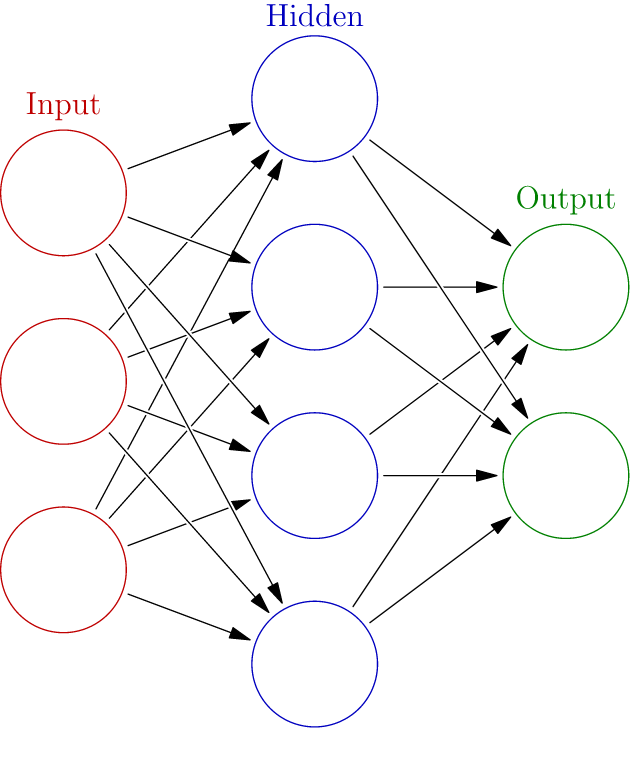
\includegraphics[width=0.45\textwidth]{images/neural_network.png}
    \cite{wiki_nn_image}
    \caption{Percettrone Multistrato}
    \label{fig:neural_network}
\end{figure}

\newpage

\subsection{Layers}

In una Rete Neurale i layers rappresentano i diversi strati della rete. In ogni strato sono presenti uno o più neuroni chiamati unità. \\

\noindent
Sono generalmente presenti tre strati :
\begin{enumerate}
    \item Input : con unità che rappresentano i campi di input.
    \item Hidden Layers : con uno o più strati.
    \item Output : con una o più unità che rappresentano i campi obiettivo.
\end{enumerate}

\noindent
I dati di input vengono presentati nel primo strato e i valori vengono propagati da ciascun neurone a ogni neurone nello strato successivo, ed alla fine viene fornito un risultato nello strato di output. \cite{ibm_neural_model}

\subsection{Pesi}

Le unità sono connesse con varie intensità di connessione, dette \hypertarget{weights}{pesi}.

Tutti i pesi inizialmente sono casuali e le risposte ottenute dalla rete risulteranno probabilmente prive di senso.

La rete apprende generando una previsione per ogni input dato e correggendo i pesi ogni volta che viene sbagliata una previsione.
Questo processo, anche detto \hyperlink{epoch}{\textit{epoca}}, viene ripetuto molte volte e la rete continua a migliorare le sue previsioni finché uno o più criteri di interruzione non vengono soddisfatti. \cite{ibm_neural_model}

\subsection{Bias}

Il parametro di \hypertarget{b}{bias} è quello che, durante il calcolo matematico che avviene all'interno della singola unità (neurone) permette di aggiungere un'errore al modello,
considerato troppo semplice, con l'obbiettivo di catturare una maggiore complessità dei dati.

\newpage

\section{Dataset}
Un Dataset è una raccolta strutturata di dati, che in questo caso servirà per la fase di addestramento (training) dei nostri modelli. \\

\noindent
In generale, un Dataset per l'addestramento di Reti Neurali è suddiviso in :
\begin{itemize}
    \item Training set : immagini usate per il training del nostro modello.
    \item Validation set : immagini utilizzate durante l'addestramento, per valutare le prestazioni del modello su dati non visti e per effettuare la messa a punto dei parametri.
    \item Test set : un insieme di immagini utilizzate alla fine dell'addestramento, per valutare le prestazioni finali del modello, su dati completamente nuovi che non sono stati utilizzati per il training.
\end{itemize}

Il Validation set è opzionale, ma molto utile per migliorare la qualità del training del modello.

\subsection{Qualità di un Dataset}
La qualità di un Dataset è data dalla correttezza delle sue annotazioni, cioè dalla coerenza di quello che mi stanno dicendo i dati al suo interno, ma anche dalla varietà dei dati al suo interno,
perché avrò molti più esempi da mostrare al mio modello nella fase di addestramento.

Perciò se i dati sono coerenti ai problemi del mondo reale di cui si occuperà il modello, impararne i pattern e le correlazioni consentirà al modello addestrato di fare previsioni accurate su nuovi dati.

\newpage

\section{Training}

L'addestramento di un modello è la fase del Machine Learning (ML) in cui avviene l'apprendimento. Nel ML, l'apprendimento implica la regolazione dei parametri di un modello ML.
Questi parametri includono \hyperlink{weights}{\textit{pesi}} e \hyperlink{b}{\textit{bias}} nelle funzioni matematiche che costituiscono i loro algoritmi.

Durante questa fase, ogni volta che un input arriva ad un nodo, viene moltiplicato per il peso (weight) associato a quella specifica connessione,
e la somma di tutti questi input con un certo valore di bias ne determinerà poi i valori in output.

Dal punto di vista matematico, l'obiettivo di questo apprendimento è quello di ridurre al minimo una funzione di perdita che quantifica l'errore degli output nelle attività di addestramento.
Quando l'output della funzione di perdita scende al di sotto di una soglia predeterminata, ovvero l'errore del modello nelle attività di addestramento è sufficientemente piccolo,
il modello viene considerato "addestrato". \cite{training_nn}

\subsection{Training from scratch}

In questa tipologia di training, il modello viene addestrato su dati annotati senza partire da pesi pre-trainati, quindi senza usare come base un modello già allenato.

Partendo da zero, ovvero from scratch, i pesi non sono definiti ma vengono assegnati dei numeri casuali che, soltanto durante il processo di training, verranno modificati per ottimizzare le prestazioni.

Questo tipo di training è valido quando abbiamo a disposizione un numero considerevole di dati annotati e l'utilizzo del modello è molto specifico.

\subsection{Transfer Learning}

In scenari caratterizzati da dataset limitati o per ottimizzare tempi e risorse computazionali, è prassi comune ricorrere al transfer learning, inizializzando la rete con pesi pre-addestrati.

Questo approccio si fonda sulla natura gerarchica dell'apprendimento profondo: i primi layer della rete estraggono caratteristiche universali delle immagini, come bordi, variazioni di colore, e texture,
mentre solo gli strati più profondi si specializzano su task specifici.
Sfruttando la rappresentazione generale appresa precedentemente su dataset massivi, si evita di dover ricostruire l'estrattore di feature da zero, concentrando il nuovo addestramento solo su ciò che è strettamente legato al nuovo dominio.

I vantaggi rispetto a un addestramento from scratch sono notevoli: una drastica riduzione dei dati annotati necessari, una convergenza più rapida, con conseguente abbattimento dei costi computazionali,
ed infine migliore capacità di generalizzazione.
Il limite principale è invece legato al cambio di dominio, dove il trasferimento di conoscenza perde di efficacia se il nuovo dominio si discosta eccessivamente da quello di partenza.

\subsection{Fine-tuning}
\label{sec:fine_tuning}

Mentre il transfer learning rappresenta il paradigma concettuale, il fine-tuning ne costituisce l'implementazione pratica, in cui l'addestramento non parte da pesi inizializzati casualmente,
ma da uno stato pre-ottimizzato che viene gradualmente adattato al nuovo dominio di riferimento.
Operativamente, si distinguono due approcci: nel fine-tuning \textit{completo} l'intera architettura viene aggiornata, garantendo massima flessibilità a fronte di un elevato onere computazionale;
nel fine-tuning \textit{parziale}, invece, i layer iniziali vengono "congelati" per preservare l'estrazione di feature generali, limitando l'aggiornamento agli strati terminali, spesso sostituiti per adattarsi alle nuove classi.

Un aspetto critico in questo processo è la calibrazione del learning rate, che deve essere sensibilmente inferiore rispetto al training from scratch.
Aggiornamenti troppo aggressivi distruggerebbero infatti i delicati equilibri dei pesi originali, innescando il cosiddetto \textit{catastrophic forgetting}, cioè la perdita irreversibile della conoscenza pregressa.
Al contempo, occorre bilanciare attentamente la durata dell'addestramento per non incappare nell'overfitting, specialmente se il nuovo dataset è di dimensioni ridotte.

Infine, l'enorme scala raggiunta dai recenti modelli linguistici e multimodali ha reso spesso quasi impraticabili gli approcci tradizionali.
Sono così emerse le tecniche di Parameter-Efficient Fine-Tuning (PEFT), che ottimizzano solo una frazione infinitesimale dei pesi mantenendo inalterata l'architettura originale.
Una delle metodologie più efficaci in questo ambito è LoRA, approfondita nella Sezione~\ref{sec:lora}.

\newpage

\section{Epoca}
Un'\hypertarget{epoch}{epoca} rappresenta un passaggio completo del dataset attraverso l'algoritmo in fase di learning, è un concetto fondamentale nel training delle reti neurali,
che permette al modello di imparare continuando costantemente a rivedere le stesse immagini, o i medesimi elementi del dataset.

Il numero di epoch si specifica solitamente in ogni procedura di training e determina quante volte il modello imparerà dal set di train del dataset, influenzando le performance e la qualità del modello.\\

\noindent
Scegliere il numero di epoch corretto è molto importante perché se viene scelto in maniera errata può creare due problemi:
\begin{itemize}
    \item Underfitting: il modello non è stato trainato per un numero sufficiente di epochs.
    Le performances non sono adeguate né sul set di training né su quello di test.
    
    \item Overfitting: il modello è stato trainato per troppi epochs.
    In questo caso memorizza i dati di training in maniera troppo approfondita e perde le sue abilità di analizzare i nuovi dati. Ha una precisione eccellente sul training set ma scarsa sul dataset di validazione.
\end{itemize}

Una tecnica comune per evitare l'overfitting è quella dell'early stopping, nella quale il training viene fermato quando le performances sul set di validazione smettono di migliorare.
A volte è possibile specificare un parametro chiamato patience, che specifica dopo quanti epochs "non migliorativi" il training deve fermarsi. \cite{epoch_ultralytics}.

	\section{Pytorch}

PyTorch è un framework di deep learning open source basato su software usato per creare reti neurali.
Combina la libreria di machine learning (ML) di Torch con un'API di alto livello basata su Python.
La sua flessibilità e facilità d'uso, tra gli altri benefici, lo hanno reso il principale framework di ML per le comunità accademiche e di ricerca.

\subsection{Tensori}

In qualsiasi algoritmo di machine learning, anche quelli applicati a informazioni apparentemente non numeriche come suoni o immagini, i dati devono essere rappresentati numericamente.
In PyTorch ciò viene ottenuto tramite tensori che fungono da unità fondamentali di dati utilizzate per il calcolo sulla piattaforma. \\

\noindent
Dal punto di vista linguistico, “tensore” è un termine generico che si riferisce ad alcune entità matematiche più familiari come :
\begin{itemize}
    \item Un vettore è un tensore monodimensionale contenente più scalari dello stesso tipo. Una tupla è un tensore monodimensionale contenente diversi tipi di dati.
    \item Una matrice è un tensore bidimensionale contenente più vettori dello stesso tipo.
    \item I tensori con tre o più dimensioni, come i tensori tridimensionali usati per rappresentare le immagini RGB negli algoritmi di computer vision, sono collettivamente denominati tensori N-dimensionali.
\end{itemize}

\noindent
Oltre a codificare gli input e gli output di un modello, i tensori di PyTorch codificano i parametri del modello: pesi e gradienti che vengono "appresi" nella machine learning.

\subsection{Grafici}
I grafici di calcolo dinamico (DCG) sono il modo in cui i modelli di deep learning vengono rappresentati in PyTorch.
Nel contesto del deep learning, questi grafici traducono essenzialmente il codice di una rete neurale in un diagramma di flusso che indica le operazioni eseguite in ciascun nodo e le dipendenze tra diversi strati nella rete, cioè la disposizione di fasi e sequenze che trasformano i dati di input in dati di output. \cite{pytorch}

	\chapter{YOLO}

YOLO, ovvero "You Only Look Once", è un diffuso algoritmo di rilevamento di oggetti in tempo reale.

YOLO unifica quello che un tempo era un processo a più fasi, utilizzando un'unica rete neurale per eseguire sia la classificazione sia la previsione dei riquadri di delimitazione (bounding box) degli oggetti rilevati.
Ogni bounding box è definita dalle coordinate che ne identificano posizione e dimensioni all'interno dell'immagine, oltre a un punteggio di confidenza e all'etichetta della classe dell'oggetto. In questo modo il modello è in grado di localizzare e classificare simultaneamente tutti gli oggetti presenti in una singola inferenza, formulando il problema come una regressione diretta delle coordinate dei bounding box e delle probabilità di appartenenza alle diverse classi.

È fortemente ottimizzato per le prestazioni di rilevamento e può operare molto più velocemente rispetto all'esecuzione di due reti neurali distinte per rilevare e classificare gli oggetti separatamente. Ciò avviene riadattando i classificatori di immagini tradizionali per la specifica attività di regressione volta a individuare i bounding box degli oggetti. \cite{yolo_info}

\newpage

\section{YOLO26}

YOLO26 è l'ultima famiglia unificata di modelli di visione in tempo reale.
Introduce l'inferenza nativa end-to-end, una head di rilevamento più leggera, una ricetta di addestramento aggiornata e head specifiche per compito per rilevamento, segmentazione, stima della posa, classificazione. \cite{yolo26_ultralytics}

\subsection{Versioni}

I modelli YOLO26, offrono diversi tagli per ogni versione del modello, passando dalla più piccola denominata "nano" (YOLO26n), alla più grande "extra large" (YOLO26x), nei quali differenza sta nella loro dimensione a livello di parametri.
Questa variazione di parametri ci permetti di aumentare le prestazioni, e quindi la qualità del modello.

\subsection{Metriche di valutazione}

Dopo aver addestrato un modello YOLO, dobbiamo misurarne le prestazioni ed eventualmente perfezionarlo per colmare le lacune.
La valutazione utilizza metriche come precision e la recall, le quali unite alla mAP ci permettono di quantificare l'accuratezza del modello. \\

\begin{table}[htbp]
    \centering
    \renewcommand{\arraystretch}{1.3}
    \begin{tabular}{lccccc}
        \toprule
        \textbf{Model} & 
        \textbf{\begin{tabular}[c]{@{}c@{}}mAP$_{50}$ \end{tabular}} &
        \textbf{\begin{tabular}[c]{@{}c@{}}mAP$_{95}$ \end{tabular}} &
        \textbf{\begin{tabular}[c]{@{}c@{}}Speed\\ \scriptsize{CPU}\\ \scriptsize{(ms)}\end{tabular}} & 
        \textbf{\begin{tabular}[c]{@{}c@{}}Speed\\ \scriptsize{GPU}\\ \scriptsize{(ms)}\end{tabular}} & 
        \textbf{\begin{tabular}[c]{@{}c@{}}params\\ \scriptsize{(M)}\end{tabular}} \\
        \midrule
        YOLO26n & 40.9 & 40.1 & $38.9 \pm 0.7$  & $1.7 \pm 0.0$  & 2.4  \\
        YOLO26s & 48.6 & 47.8 & $87.2 \pm 0.9$  & $2.5 \pm 0.0$  & 9.5  \\
        YOLO26m & 53.1 & 52.5 & $220.0 \pm 1.4$ & $4.7 \pm 0.1$  & 20.4 \\
        YOLO26l & 55.0 & 54.4 & $286.2 \pm 2.0$ & $6.2 \pm 0.2$  & 24.8 \\
        YOLO26x & 57.5 & 56.9 & $525.8 \pm 4.0$ & $11.8 \pm 0.2$ & 55.7 \\
        \bottomrule
    \end{tabular}
\end{table}
\cite{yolo26_ultralytics}

\newpage

\subsubsection{Precision}
La precision è la frazione di istanze rilevanti tra le istanze recuperate.

$$ Precision =\frac{\text{Istanze rilevanti recuperate}}{\text{Tutte le istanze recuperate}} = \frac{TP}{TP+FP} $$

\subsubsection{Recall}
La recall (anche nota come sensibilità) è la frazione di istanze rilevanti che sono state recuperate.

$$ Recall =\frac{\text{Istanze recuperate rilevanti}}{\text{Tutte le istanze rilevanti}} = \frac{TP}{TP+FN} $$

\noindent  \\ \\
Sia la precision che la recall si basano sull'output generato dal nostro modello. Queste metriche possono essere meglio rappresentate tramite questa immagine. 
\begin{figure}[htbp]
  \centering
  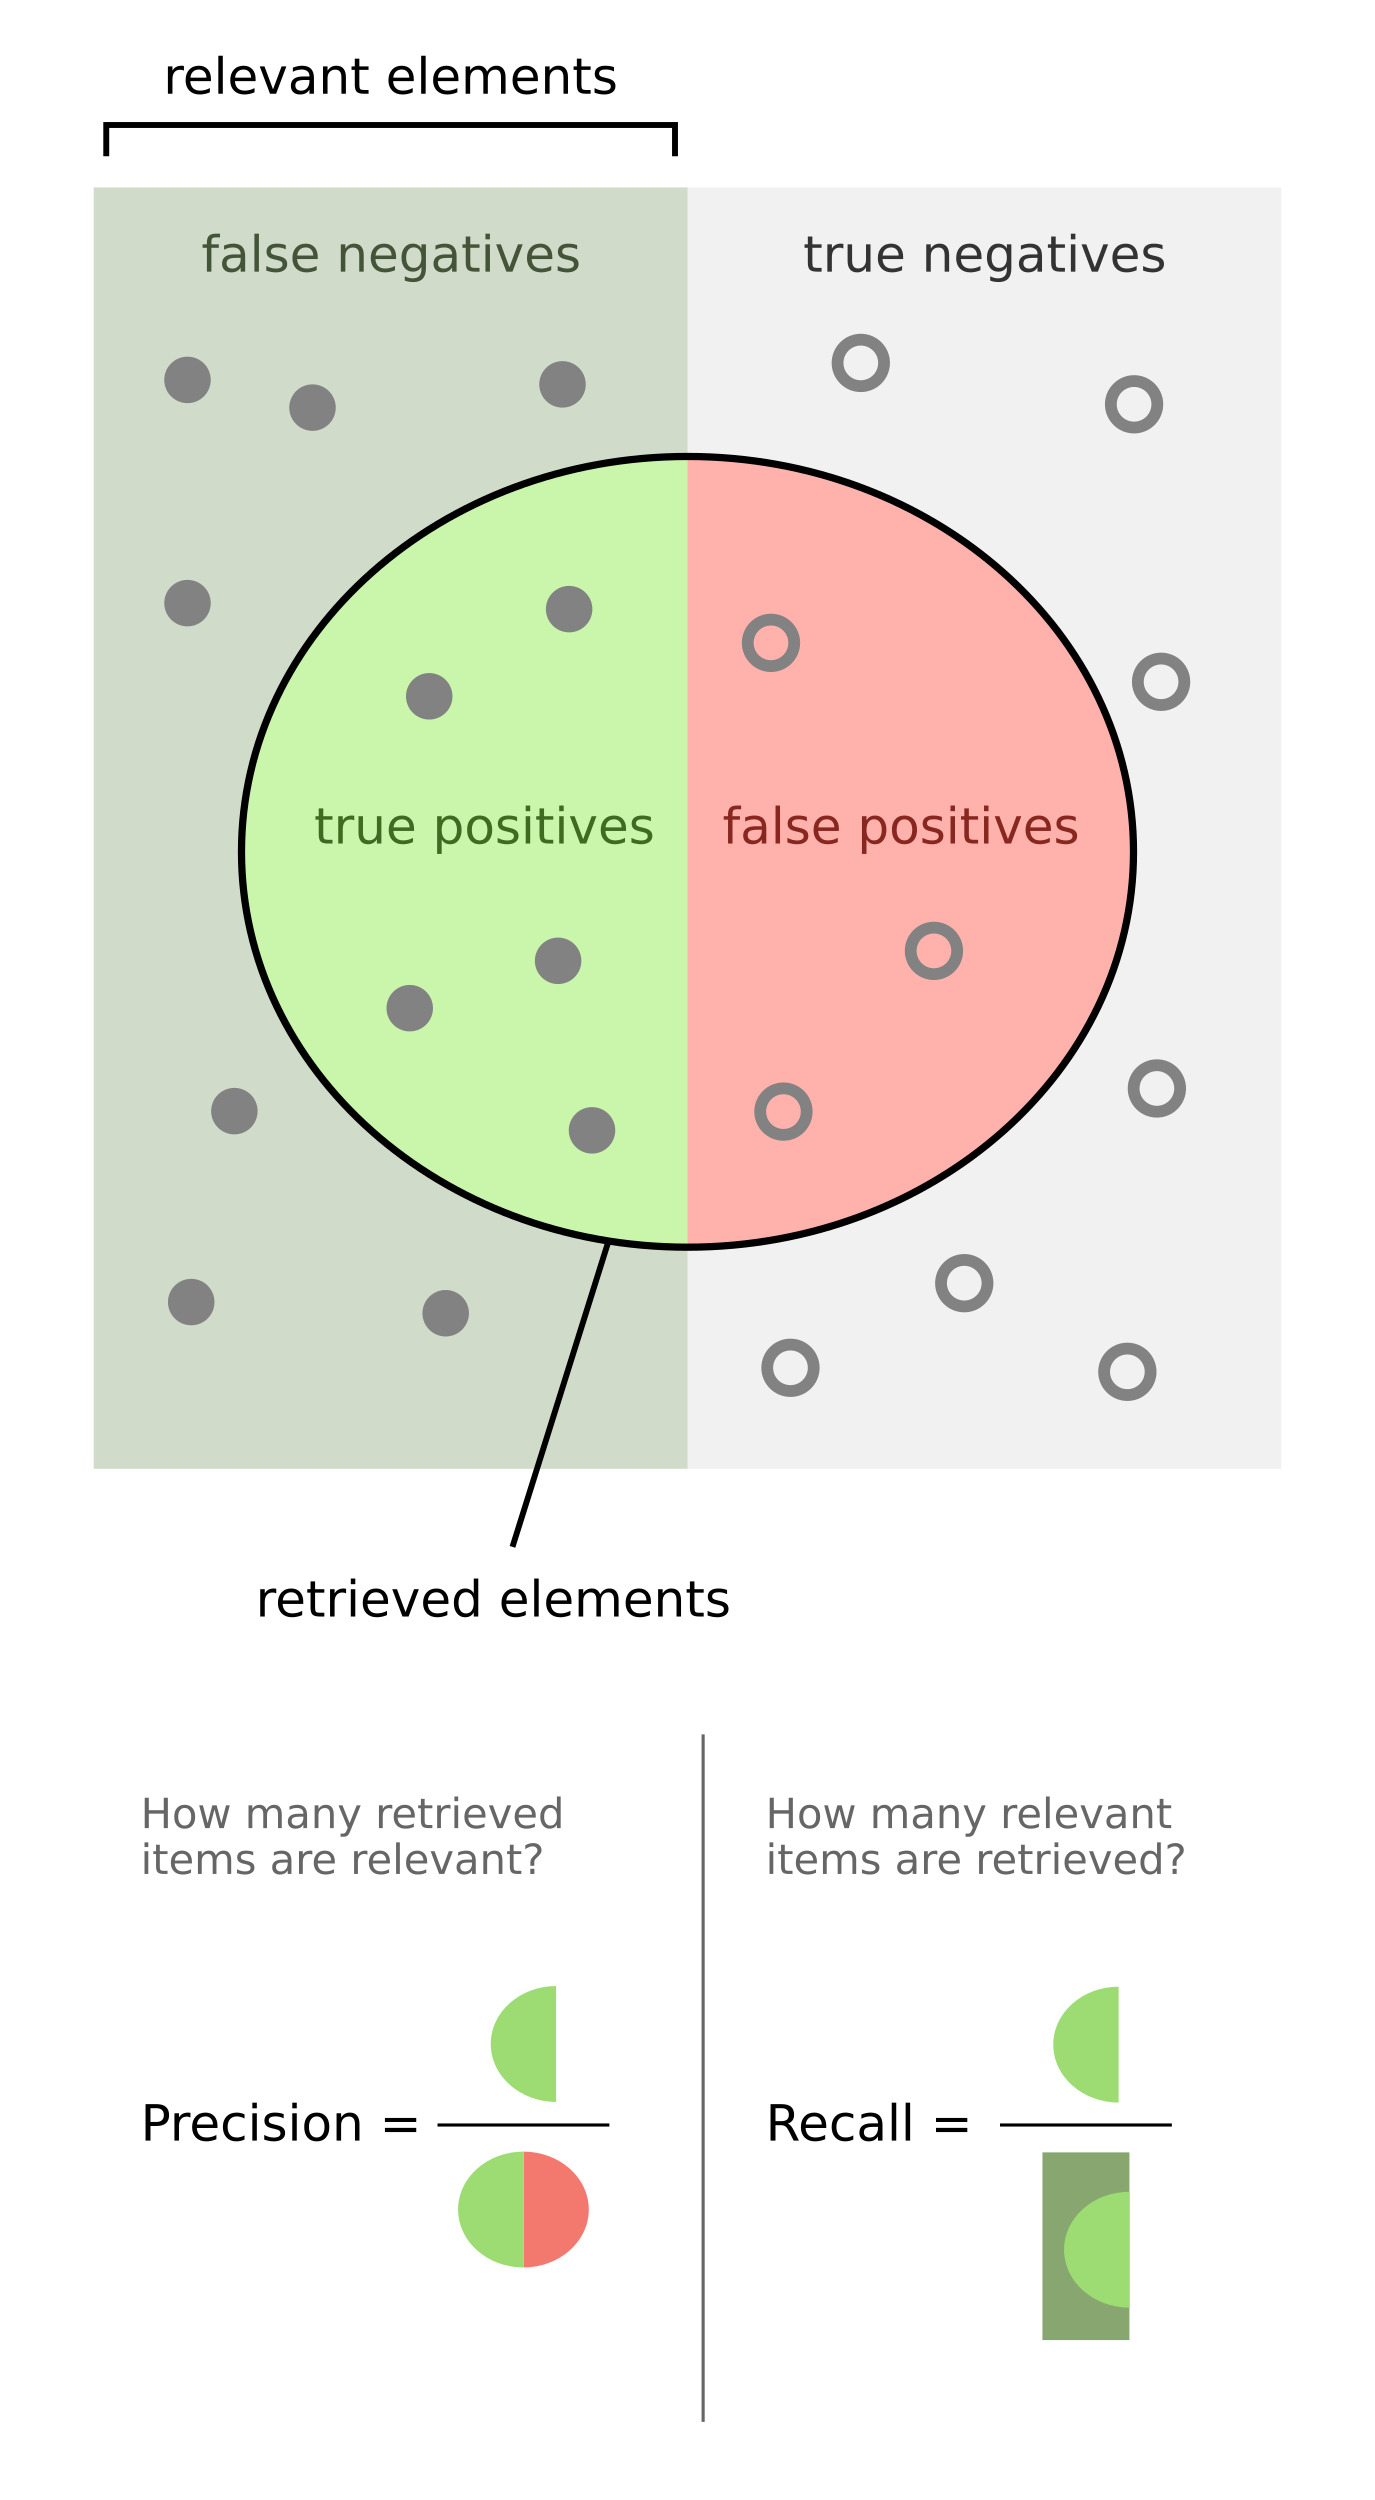
\includegraphics[width=0.8\textwidth]{images/precision-recall.jpg}
  \cite{precision_recall}
  \label{fig:precision_recall}
\end{figure}

\subsubsection{F1 score}
L'F1 score mette in rapporto tra la precision e la recall, offrendoci una migliore comprensione del bilanciamento del nostro modello.

\newpage

\subsubsection{mAP}
La precisione media (mean average precision) è una metrica di apprendimento automatico progettata per valutare gli algoritmi di rilevamento degli oggetti.

Negli articoli scientifici relativi al rilevamento di oggetti, è possibile imbattersi in abbreviazioni come  \(mAP_{50}\) o \(mAP_{95}\). In breve, questa notazione indica la soglia IoU utilizzata per calcolare l'mAP.

\subsubsection{IoU}
L'Intersection over Union viene calcolato dividendo la sovrapposizione tra l'annotazione prevista e quella reale per l'unione di queste due.
\begin{figure}[htbp]
  \centering
  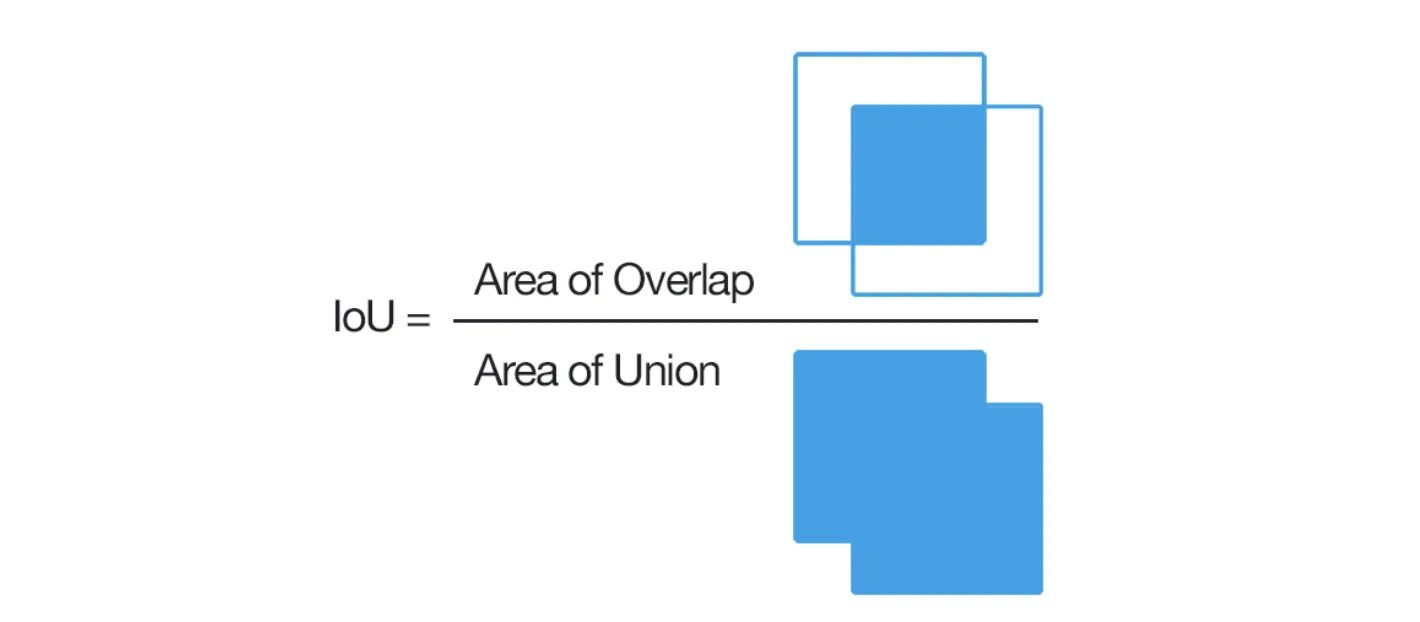
\includegraphics[width=0.8\textwidth]{images/IoU.jpg}
  \cite{IoU}
  \caption{Intersection over Union}
  \label{fig:IoU}
\end{figure}

\noindent
Per capire meglio, ecco alcuni esempi :
\begin{itemize}
    \item Se impostassimo la soglia IoU a 0,9, e la precision fosse pari al 16\% vorrà dire che solo 1 previsione su 6 corrisponde al punteggio;

    \item Con una soglia pari a 0,7, ed una precision del 65\% avrò che 4 previsioni sono al di sopra di tale punteggio.

    \item E se la soglia fosse del 0,3, e la precision salisse al 100\% vuol dire che tutte le previsioni hanno un IoU superiore a 0,3.
\end{itemize}

\noindent
Pertanto, la soglia IoU può influenzare significativamente il valore medio finale della Precisione Media. Questa dipendenza introduce variabilità nella valutazione del modello. Questo è negativo, perché può verificarsi uno scenario in cui un modello ottiene buoni risultati con una determinata soglia IoU e prestazioni nettamente inferiori rispetto ad un'altra.

Per contrastare questa debolezza, si è deciso di misurare la Precisione Media per ogni classe e per ogni soglia IoU, per poi calcolare la media dei punteggi ottenuti. \cite{mAP}

\section{Script}
Di seguito sono definite le operazioni necessarie, e specifiche per l'addestramento del modello base per la object detection YOLO26n.

\subsection{Dataset}
Il dataset utilizzato per il training di questo specifico modello YOLO è composto da una serie di immagini contenenti vari capi d'abbigliamento. Nello specifico, le annotazioni di questo dataset sono state generate tramite un ulteriore modello di segmentazione, chiamato SAM3, che verrà approfondito in seguito. \\
\noindent
Per la fase di inferenza è stato invece impiegato un dataset più ridotto. Poiché quest'ultimo comprendeva inizialmente alcune immagini già presenti nel set di training, è stata effettuata un'operazione di pulizia dei dati: tali immagini sono state rimosse dal dataset di addestramento, garantendo così una maggiore affidabilità nella valutazione qualitativa del modello.

\subsection{Training}

\subsubsection{Inizializzazione}

\begin{lstlisting}
import ultralytics
from ultralytics import YOLO
\end{lstlisting}

\subsubsection{Elaborazione}

\begin{lstlisting}
model = YOLO("yolo26n.pt")

trainArgs = {
    'data' : "dataset/dataset.yaml",
    'epochs' : 100,
    'imgsz' : 640,
    'batch' : 64,
    'device' : 0,
    'name' : "detection",
    'workers' : 4,
    'patience' : 10,
    'plots' : True,
}

model.train(**trainArgs)
\end{lstlisting}

\subsubsection{Parametri}
Dei parametri utilizzati nell'addestramento, i più rilevanti per le prestazioni sono :
\begin{itemize}
    \item epochs : numero di epoche
    \item batch size : numero di immagini alla volta che gli passo
    \item device : hardware che voglio utilizzare
    \item workers : numero di "lavoratori" CPU che mi aiutano in questo processo
\end{itemize}

\subsection{Risultati}
Alla fine della fase di addestramento, verranno prodotte delle statistiche che ci serviranno per la valutazione del nostro modello, cioè la precision, recall, F1 score e l'mAP.

\begin{figure}[htbp]
  \centering
  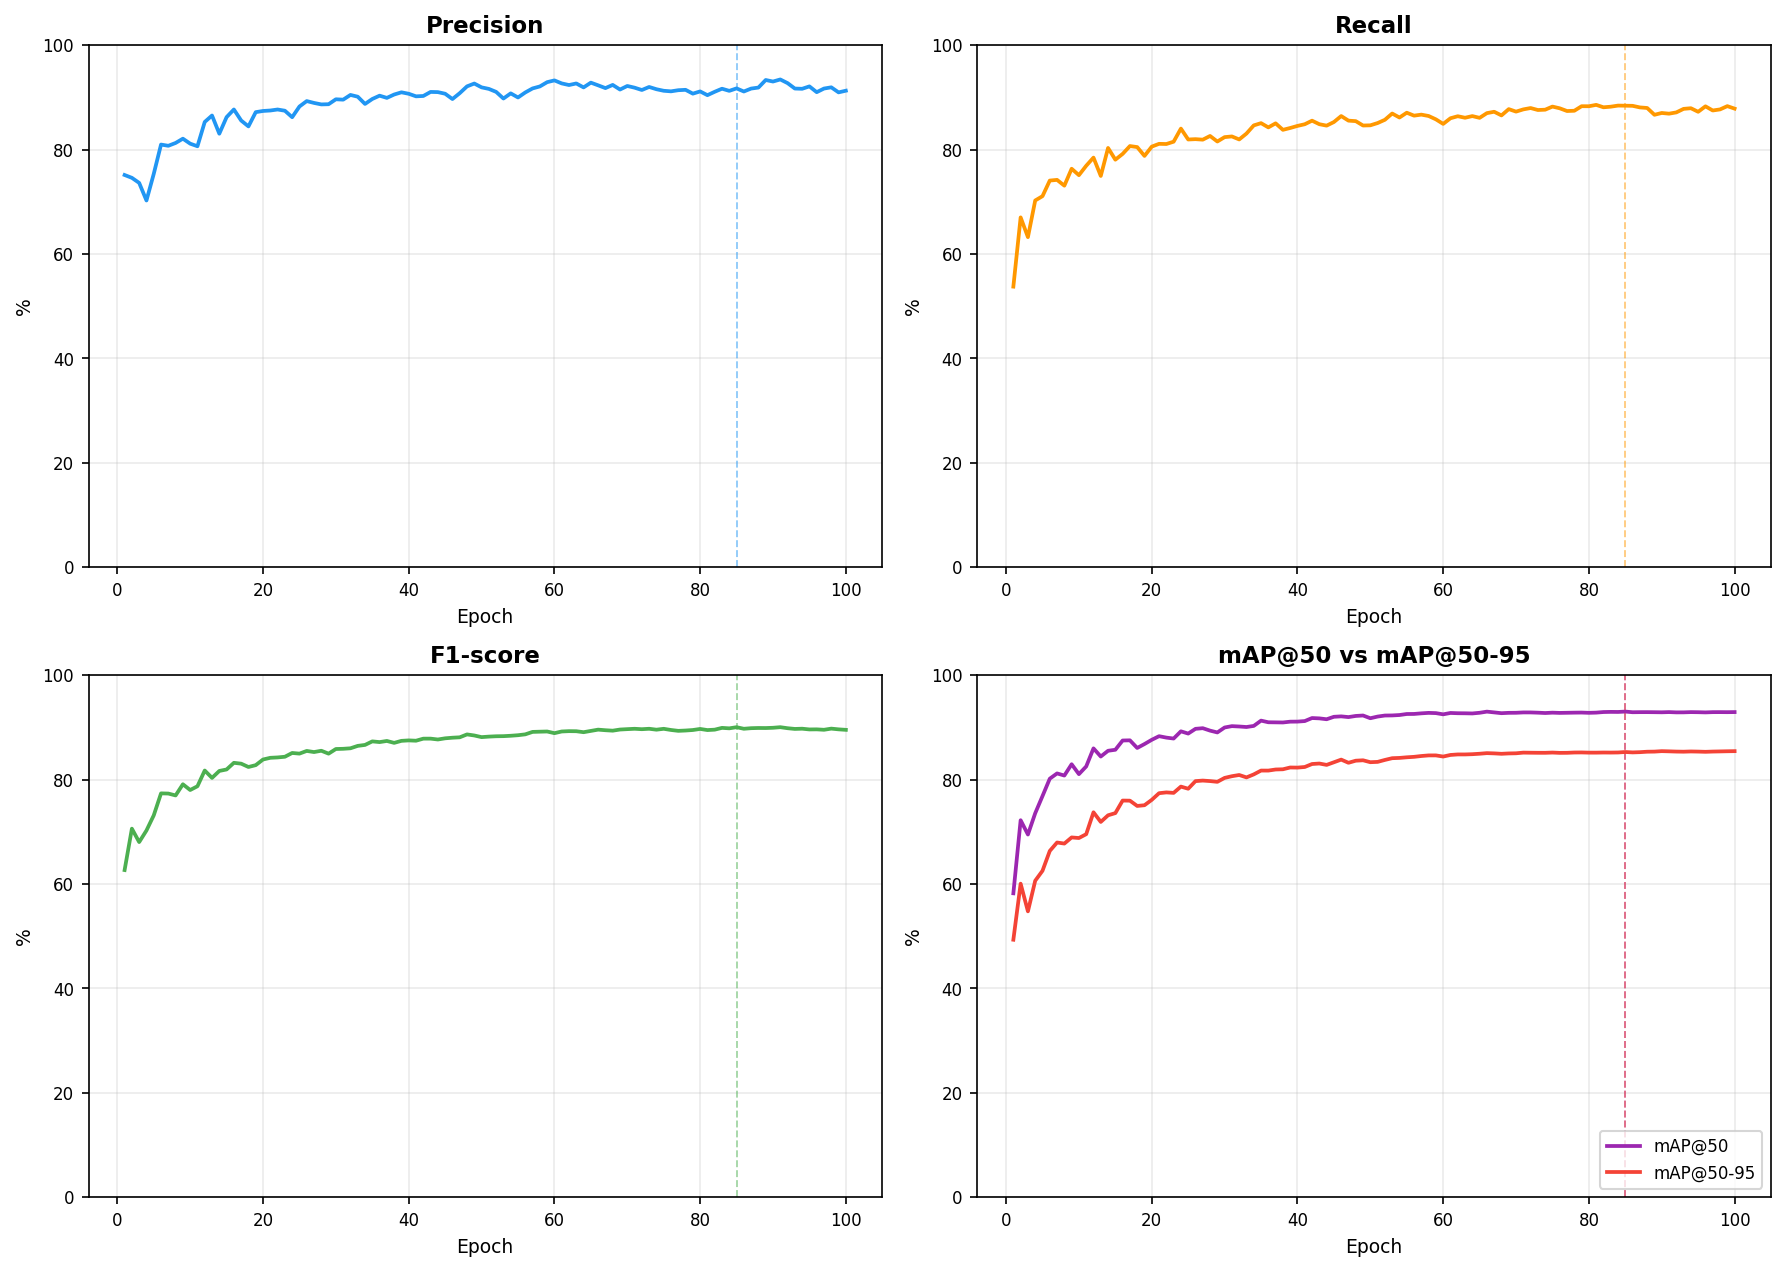
\includegraphics[width=0.8\textwidth]{images/training YOLO26n/training-stats.png}
  \caption{statistiche}
  \label{fig:statistiche}
\end{figure}

\noindent
Possiamo notare come inizialmente i grafici siano più rumorosi, e come invece più si va avanti nel numero di epoche, più la curva si stabilizzerà raggiungendo il suo plateau.

\newpage

\subsubsection{Confidence}
È il livello minimo di confidenza entro il quale il modello considera l'oggetto come valido. Questo è ottenuto andando a guardare il risultato dell'IoU e controllando che sia al sopra di questa soglia minima, che solitamente è impostata di default al 50\%. \\

\begin{figure}[h!]
  \centering
  \begin{minipage}[b]{0.49\textwidth}
    \centering
    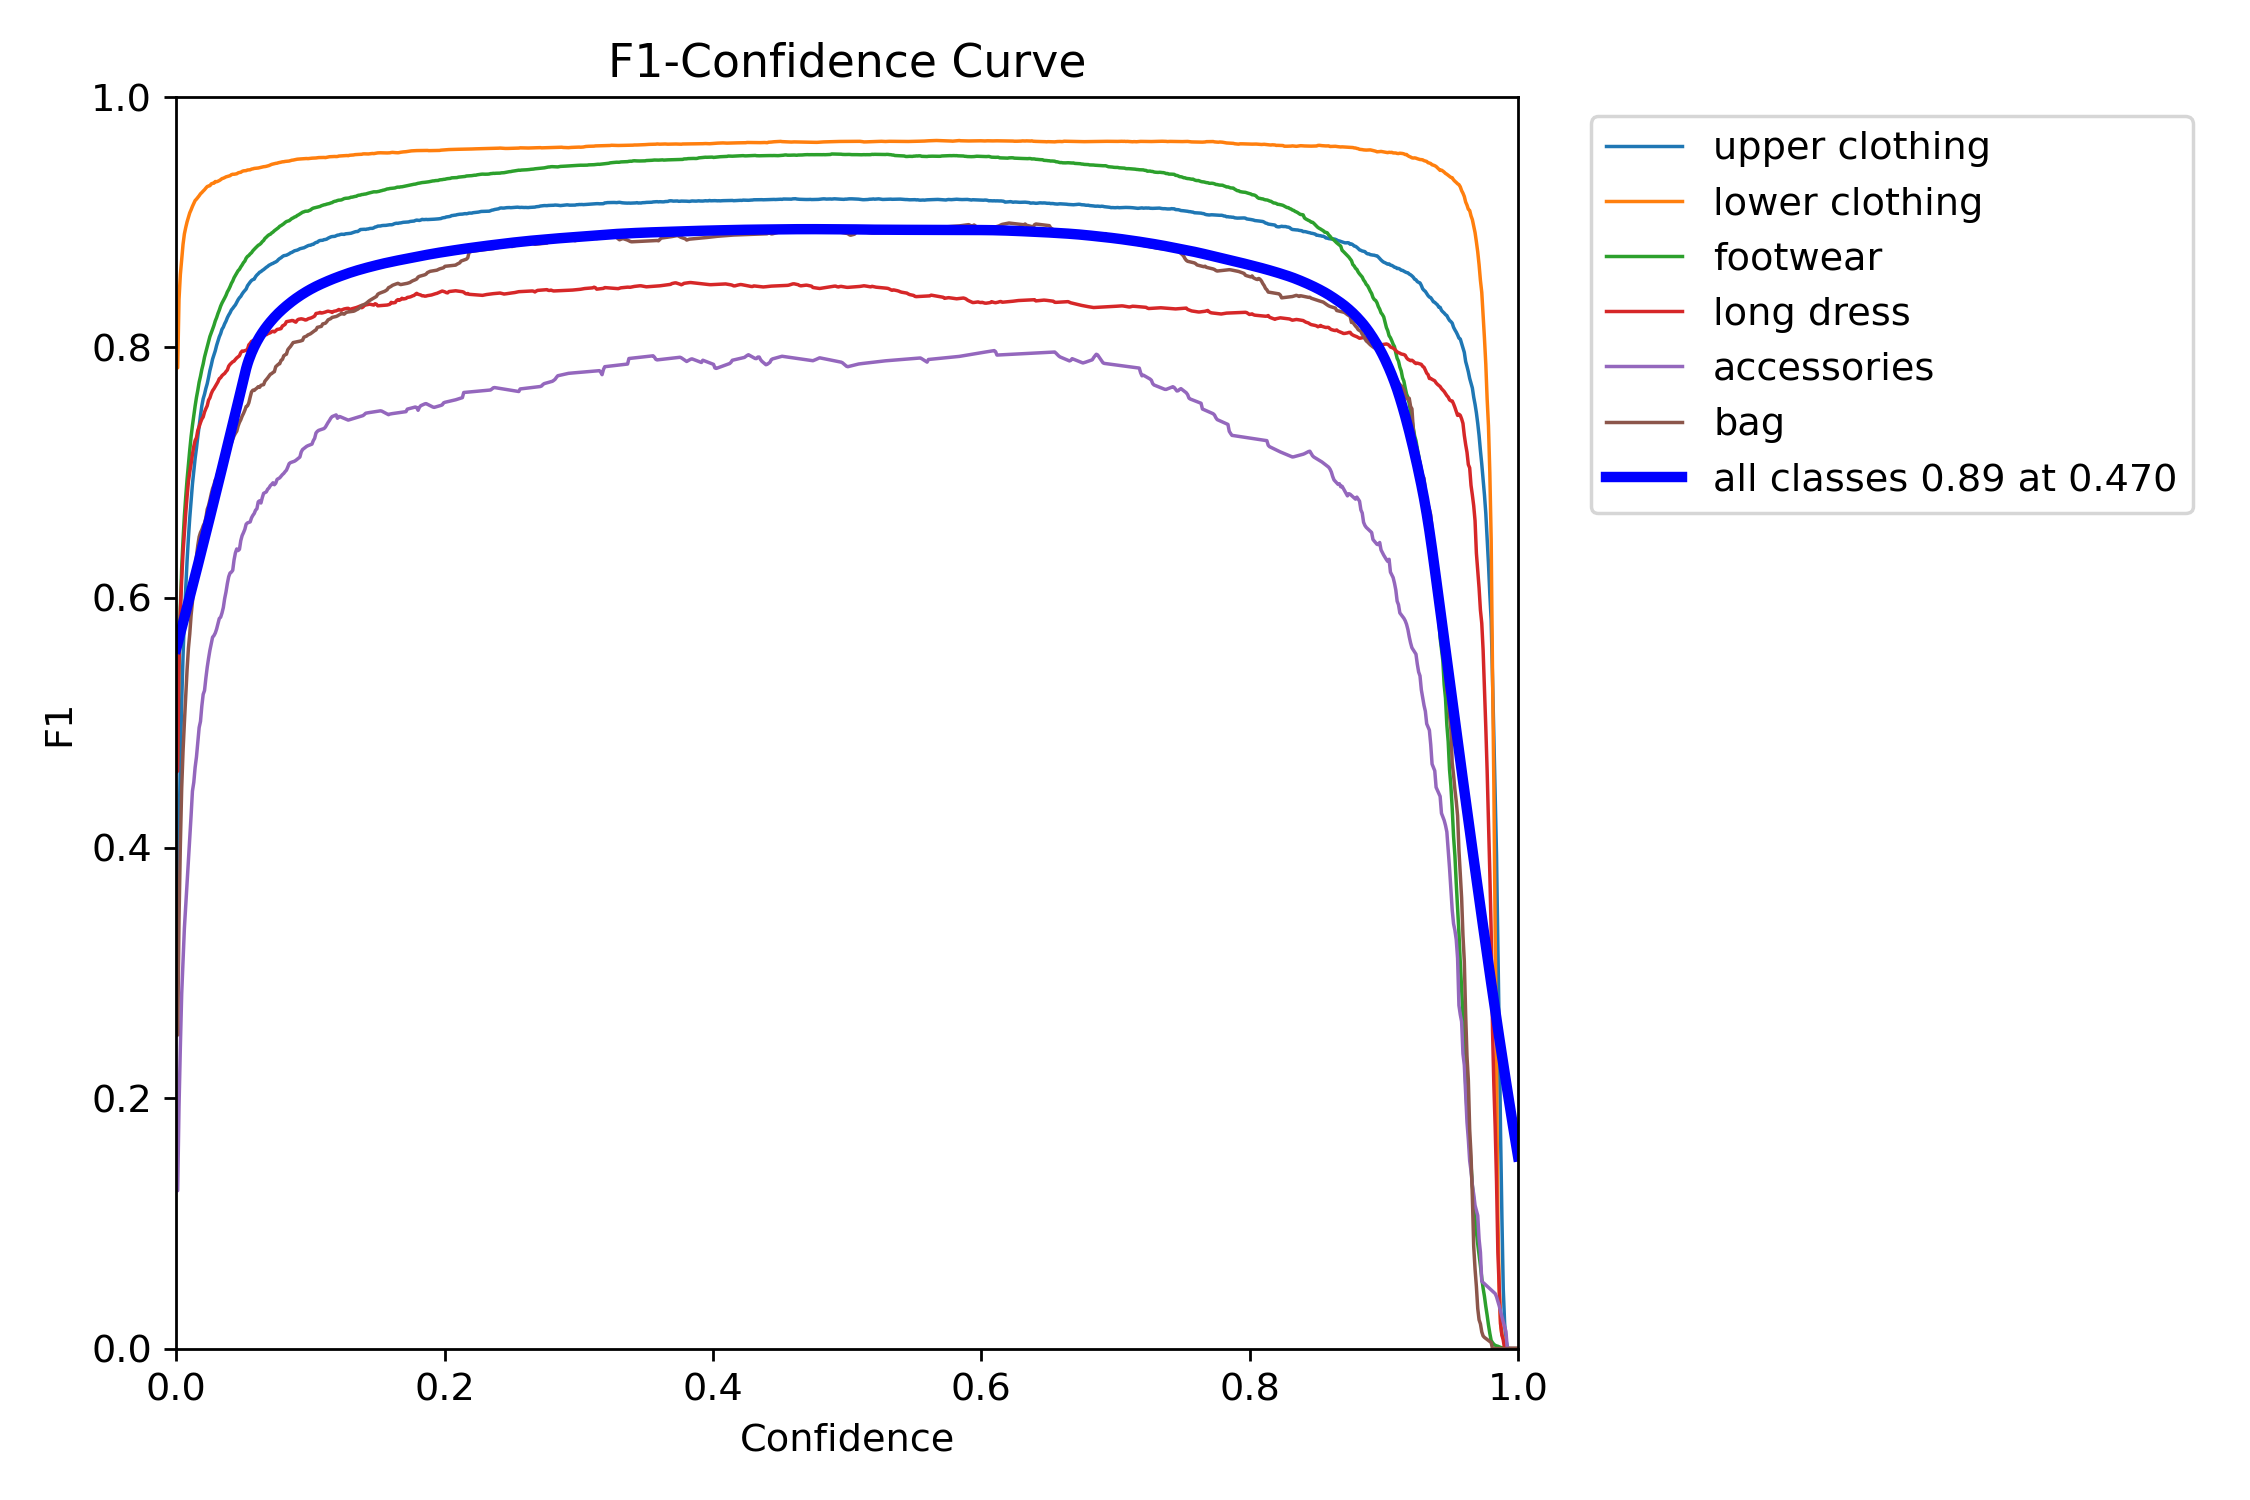
\includegraphics[width=\textwidth]{images/training YOLO26n/BoxF1_curve.png}
    \label{fig:f1_curve}
  \end{minipage}
  \hfill
  \begin{minipage}[b]{0.49\textwidth}
    \centering
    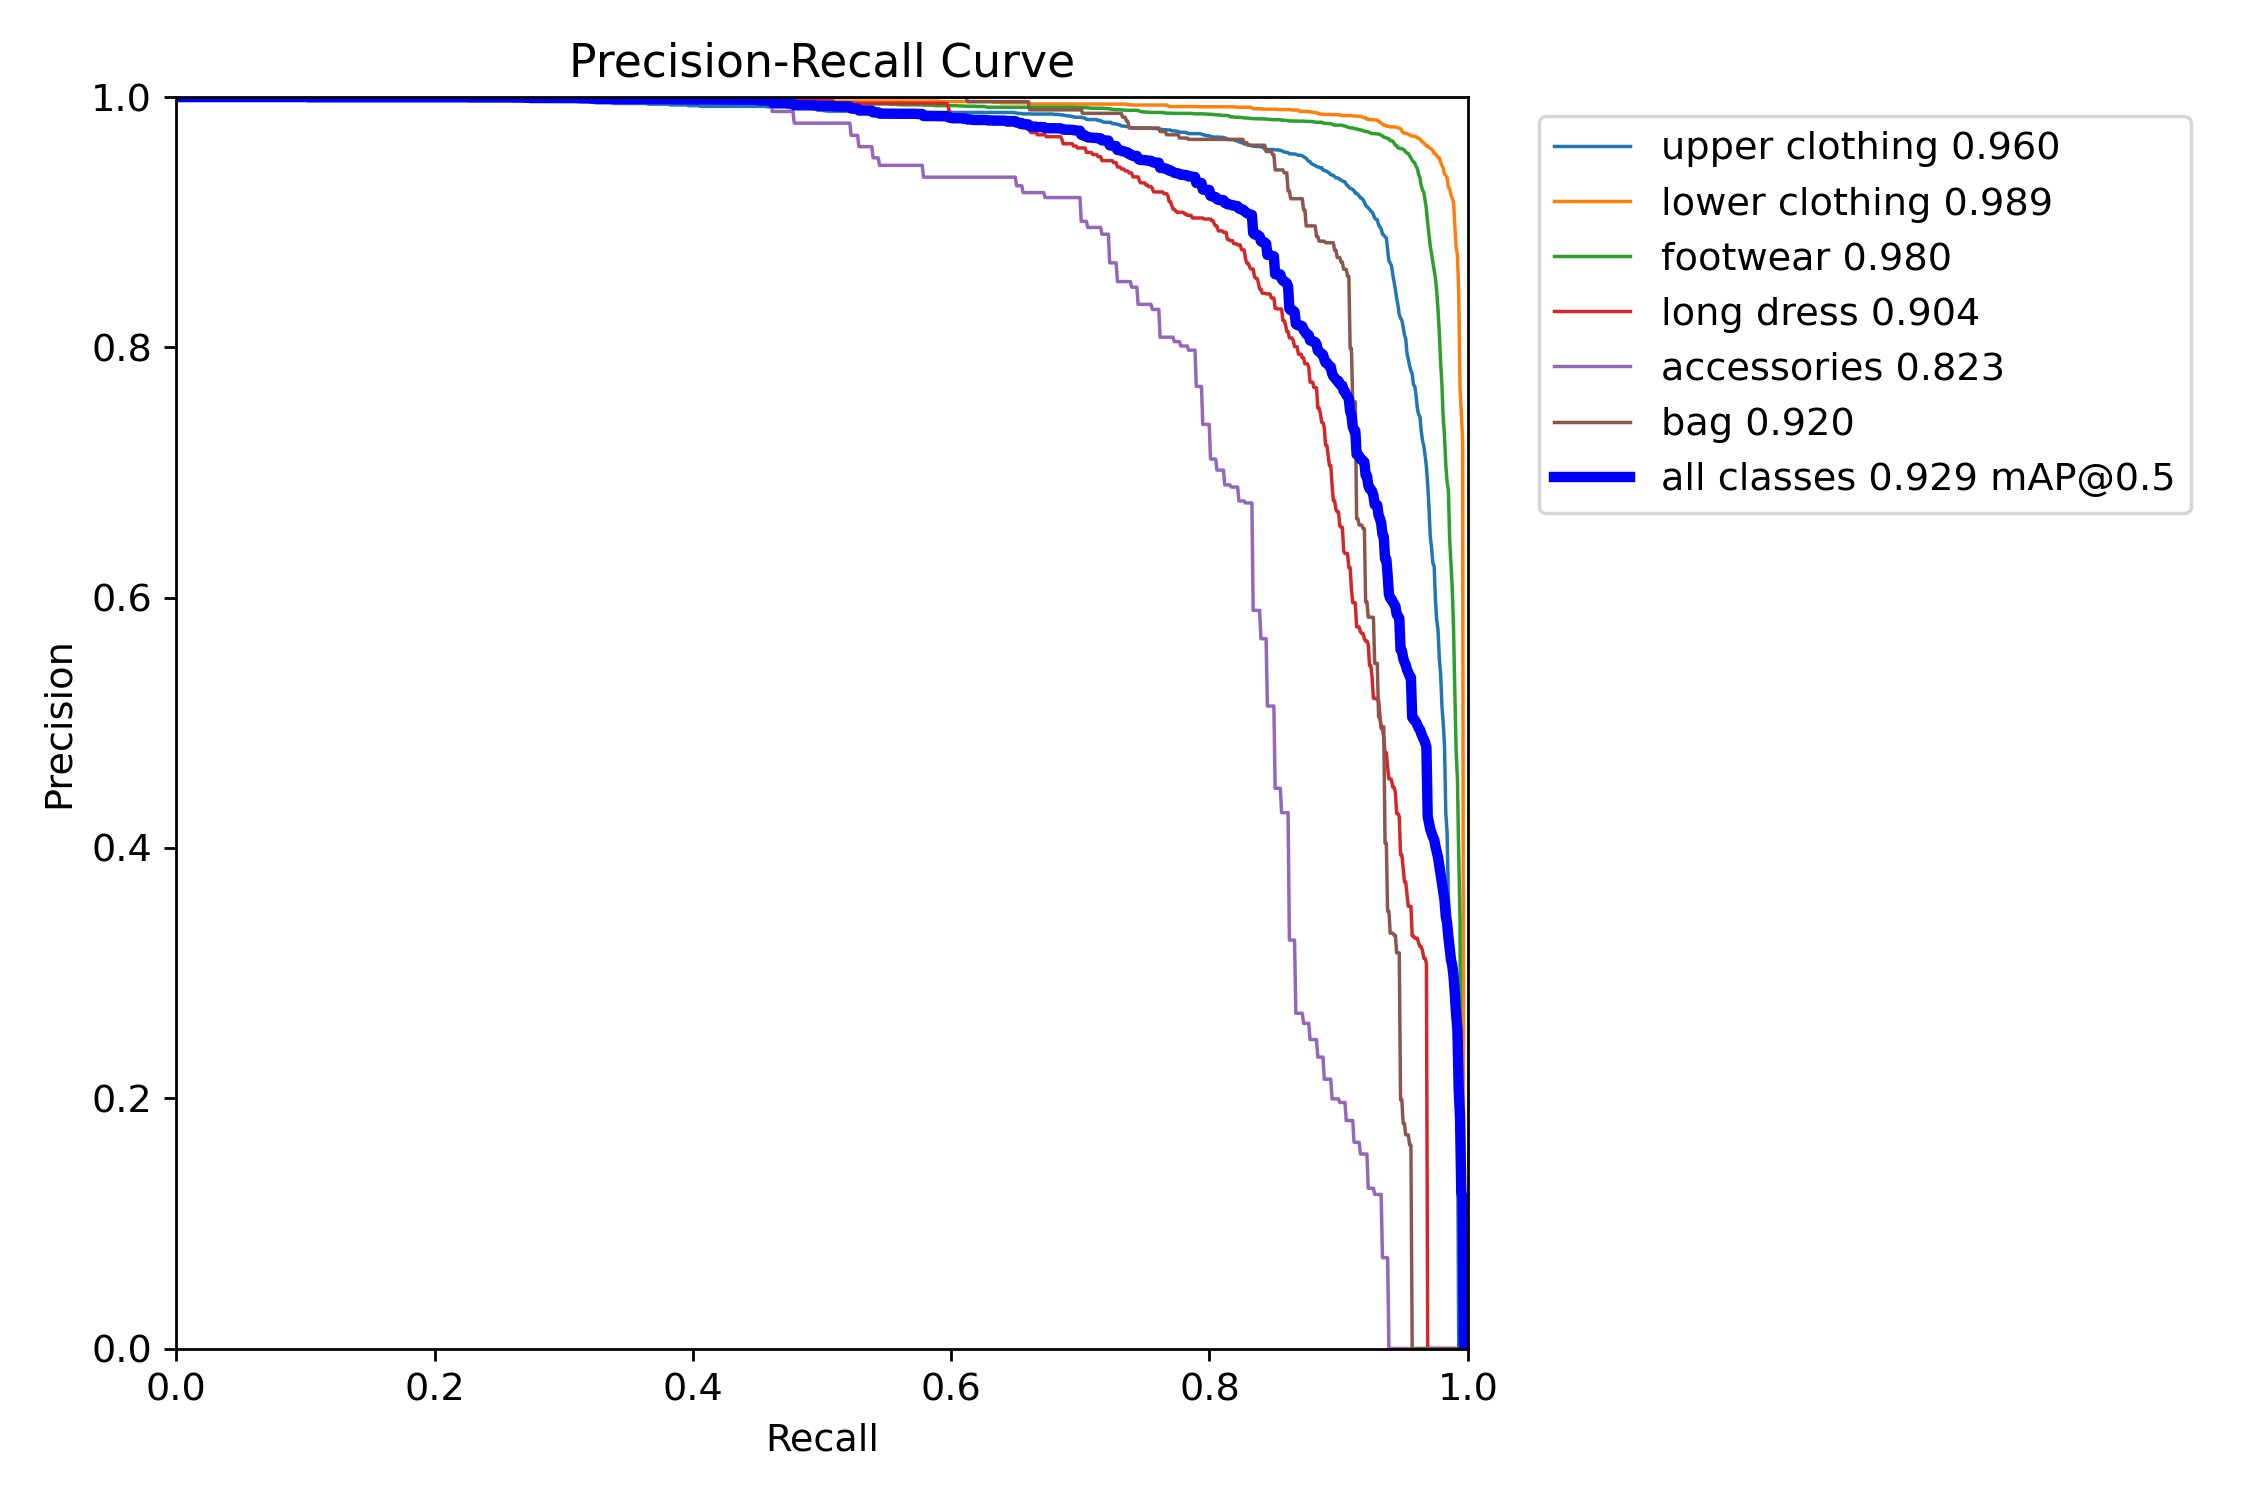
\includegraphics[width=\textwidth]{images/training YOLO26n/BoxPR_curve.png}
    \label{fig:pr_curve}
  \end{minipage}
\end{figure}

\noindent
Nel grafico a sinistra possiamo vedere che il punto massimo della curva F1, la quale rappresenta il punto ottimale in cui la soglia di confidence  fornisce il miglior compromesso tra precision e recall, è di 0.89 ottenuto  con confidence 0.470. \\
\noindent
Quindi il miglior bilanciamento tra la precision e la recall si otterrà impostando una confidence, cioè un limite di soglia, pari al 47\%.
Questo grafico è molto importante per scegliere il valore di confidence da fornire in fase di inferenza, dove appunto si minimizzano il più possibile i fenomeni di falso positivo (precision) e falso negativo (recall). \\

\noindent
In quello a destra, invece mostra la relazione fra precision e recall, con un valore di mAP50 pari a 0.929, e indica la media della precision agli intervalli di recall per tutte le classi, alla soglia di IoU di 0.5. \\
\noindent
In sostanza evidenzia il bilanciamento tra la capacità del modello di identificare in maniera corretta oggetti (precision) e la capacità di trovarli tutti (recall) per i vari livelli di soglia di confidenza.

\newpage

\subsubsection{Confusion matrix}

La confusion matrix mostra come il modello classifica le classi su cui è stato addestrato. \\

\begin{figure}[h!]
  \centering
  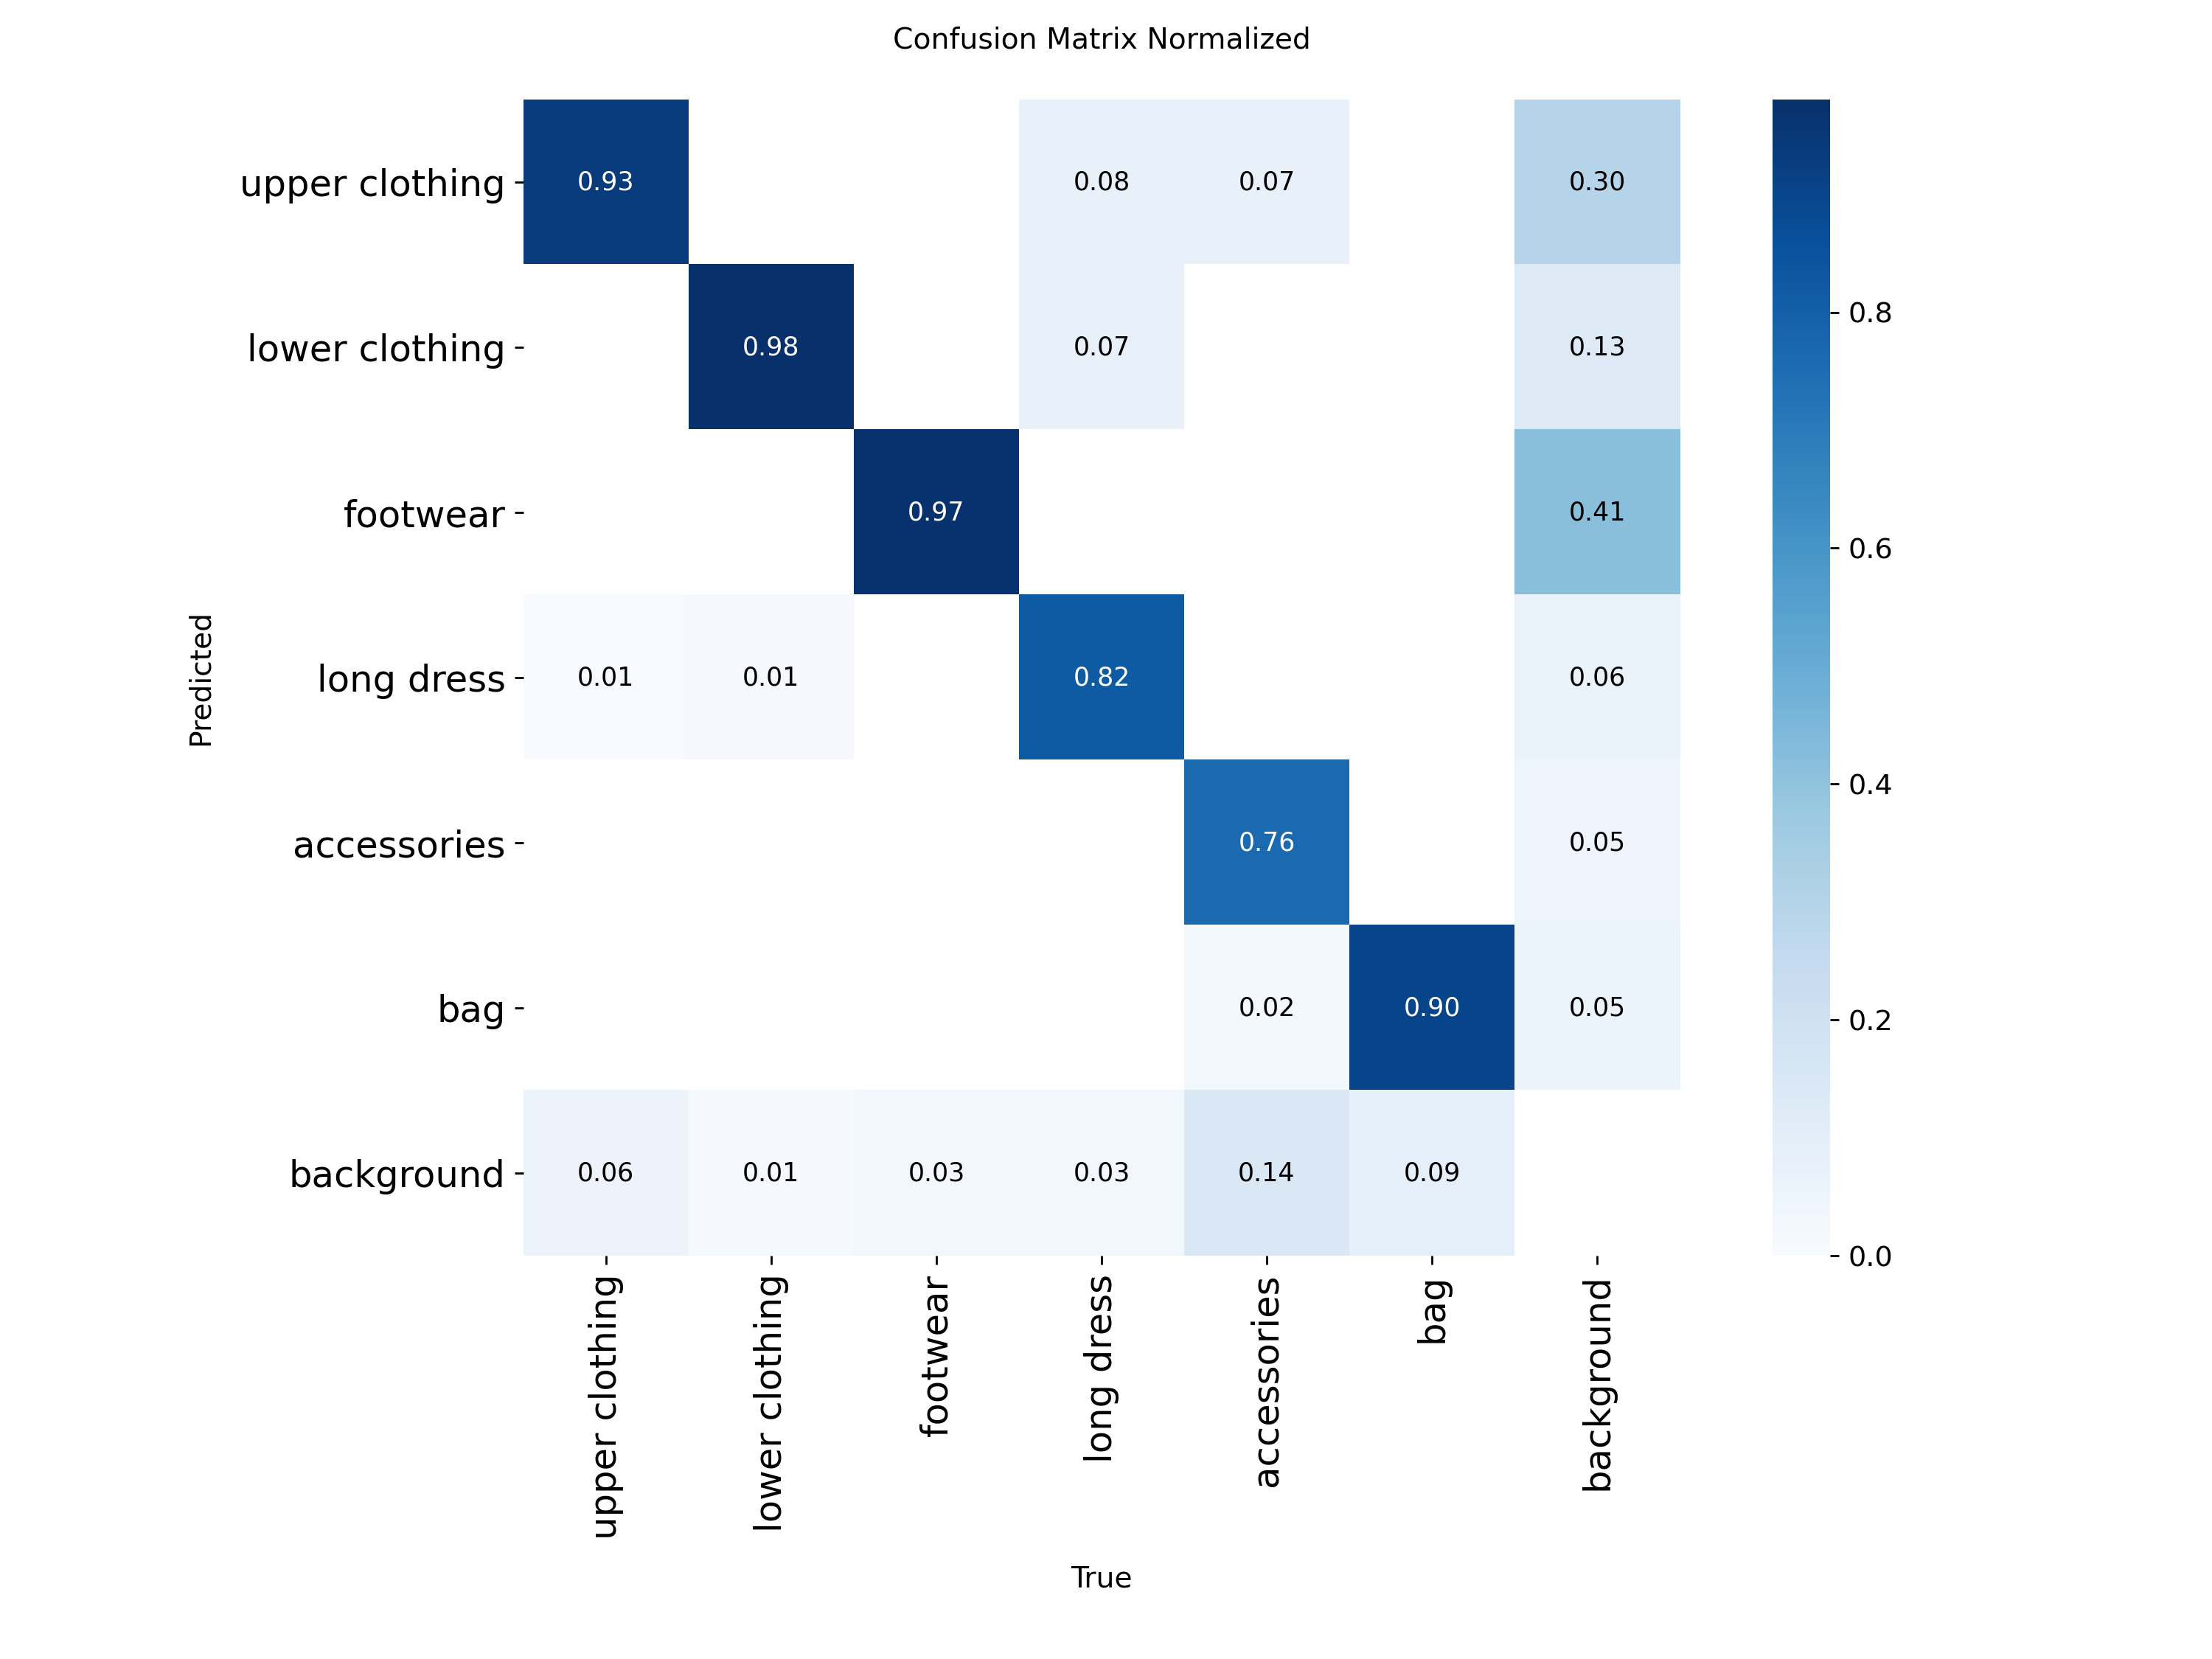
\includegraphics[width=0.8\textwidth]{images/training YOLO26n/confusion_matrix_normalized.png}
  \label{fig:confusion_matrix}
\end{figure}

\noindent
Il grafico può essere riassunto con alcune delle sue classi come :

\begin{itemize}
    \item Predicted "upper clothing" | True "upper clothing" : \\
        - il modello ha identificato correttamente il 93\% della categoria "upper clothing.
    \item Predicted "background" | True "accessories" : \\
        - il 14\% degli accessori è stato classificato come "background" (falso negativo).
    \item Predicted "footwear" | True "background" : \\
        - il 41\% del "background" è stato classificato come tale (vero negativo).
    \item Predicted "background" | True "background" : \\
        - nessun "background" è stato erroneamente classificato come capo d'abbigliamento (falso positivo assente).
\end{itemize}

\newpage

\subsection{Inferenza}

Dopo aver addestrato il modello con il nostro dataset, è possibile procedere con l'inferenza su altre immagini per verificare la presenza di alberi. Importante è soprattutto fare l'inferenza su un dataset diverso da quello utilizzato nella fase di training,, così da ottenere dei risultati più veritieri. \\
\noindent
È importante assicurarsi che le immagini in input siano dello stesso formato di quelle preparate per il training, in questo caso 640x640, devono quindi rispettare la risoluzione e la composizione dei channels RGB. \\

\noindent
Qui di seguito è dettagliata la funzione Python per l'inferenza con YOLO di Ultralytics, tramite la libreria OpenCV utilizzata in questo caso per lavorare con le immagini in input e output. \\

\begin{lstlisting}
def run(modelPath, imagesDir, outputDir="predictions", conf=0.25):
    model = YOLO(modelPath)
    Path(outputDir).mkdir(parents=True, exist_ok=True)

    for imgPath in Path(imagesDir).iterdir():
        img = cv2.imread(str(imgPath))
        if img is None:
            continue

        for result in model(img, conf=conf):
            for box in result.boxes.xyxy.cpu().numpy().astype(int):
                x1, y1, x2, y2 = box
                cv2.rectangle(img, (x1, y1), (x2, y2), (0, 255, 0), 2)

        cv2.imwrite(f"{outputDir}/{imgPath.stem}_result.jpg", img)
\end{lstlisting}

\vspace{0.5cm}
\noindent
Questa funzione implementa la fase di inferenza del modello YOLO26 su un insieme di immagini. Dato il percorso dei pesi addestrati e quello della cartella di input, il modello viene caricato tramite la libreria Ultralytics e applicato iterativamente a ciascuna immagine, con una soglia di confidenza configurabile che filtra le predizioni meno affidabili. \\
\noindent
Per ogni immagine vengono estratte le bounding box predette, sovrapposte all'immagine originale e il risultato viene salvato in una cartella di output dedicata, consentendo così una verifica qualitativa delle detection prodotte dal modello.

	\chapter{SAM3}

Il Segment Anything Model 3 (SAM 3) è un modello foundation di computer vision sviluppato da Meta e integrato nella libreria Ultralytics, progettato per compiti di rilevamento, segmentazione di istanze (instance segmentation) e tracciamento di oggetti all'interno di sequenze video. Rispetto alle versioni precedenti (SAM 1 e SAM 2), le quali limitavano la segmentazione a un singolo oggetto individuato tramite prompt visivi puntuali (come coordinate o riquadri delimitatori), SAM 3 introduce il paradigma della Promptable Concept Segmentation (PCS). Grazie a questo approccio a vocabolario aperto (open-vocabulary), il modello è in grado di identificare e segmentare contemporaneamente tutte le istanze appartenenti a un determinato concetto visivo presente nella scena. Tali concetti possono essere specificati tramite descrizioni in linguaggio naturale (es. "gatto a strisce"), esemplari visivi di riferimento o combinazioni di entrambi.

Dal punto di vista architetturale, SAM 3 disaccoppia la fase di riconoscimento da quella di localizzazione mediante l'uso di un token di presenza globale. Il sistema separa nettamente il modulo di rilevamento — basato su un'architettura di tipo DETR con fusion encoder — dal tracker video con memoria ereditato da SAM 2. Addestrato sul vasto dataset SA-Co (comprendente oltre 5 milioni di immagini e 1,4 miliardi di maschere), SAM 3 raggiunge prestazioni allo stato dell'arte con un raddoppio dell'efficienza nella segmentazione per concetto e un tempo medio d'inferenza di circa 30 ms per immagine. \cite{sam3}

\newpage

\section{Generazione del Dataset}

Inizialmente si era partiti da un insieme primario di immagini privo delle annotazioni necessarie per l'addestramento dei modelli di object detection. Date le elevate capacità di generalizzazione e accuratezza di SAM 3, il modello è stato impiegato come strumento di annotazione automatica (pseudo-labeling) per la costruzione del dataset finale.

Nello specifico, la funzionalità PCS ha consentito di estrarre le regioni d'interesse fornendo in input al modello le immagini accompagnate da prompt testuali descrittivi delle varie categorie di capi d'abbigliamento da identificare. L'elaborazione ha prodotto per ciascuna immagine le relative maschere di segmentazione per le istanze rilevate.

Poiché l'obiettivo finale risiedeva nell'addestramento del modello di object detection YOLO26 — il quale richiede in input delimitatori rettangolari (bounding box) anziché maschere poligonali — si è proceduto alla conversione sintetica delle annotazioni: a partire dai contorni di ciascuna maschera generata da SAM 3, sono state calcolate le coordinate estreme per ricavare i bounding box corrispondenti. Tale procedura ha permesso di trasformare efficacemente un processo di segmentazione di istanze in un dataset strutturato per l'addestramento di modelli di object detection.

\section{Script}

Lo script realizza un annotatore automatico: prende in ingresso una cartella di immagini prive di etichette e produce in uscita un dataset di object detection in formato YOLO, senza alcun intervento manuale. Il ruolo di SAM3 è quello di annotatore zero-shot: non viene addestrato né adattato al dominio, ma viene interrogato in linguaggio naturale con i nomi delle classi che si vogliono ottenere.
L'annotazione umana, che è la voce di costo dominante nella costruzione di un dataset, viene sostituita dalla definizione di una lista di prompt testuali.

Un punto concettuale importante è che SAM3 è un modello di segmentazione, quindi restituisce maschere a livello di pixel.
La detection non è quindi un output nativo del modello, ma una proiezione: la maschera è la rappresentazione intermedia da cui si ricava la bounding box. Questo spiega perché lo stesso identico flusso possa alimentare, senza costi aggiuntivi di inferenza, anche un dataset di segmentazione semantica.

\newpage

\subsection{Librerie}

\begin{lstlisting}
import shutil
import torch

from pathlib import Path
from PIL import Image
from transformers import Sam3Model, Sam3Processor
\end{lstlisting}

\subsection{Configurazione}

Tutto ciò che definisce il dataset è dichiarativo: le cartelle di input e output, l'elenco delle classi e le soglie. L'ordine di CLASSES definisce implicitamente il class\_id numerico usato nelle annotazioni YOLO.

CLASS\_PROMPTS introduce una distinzione utile da sottolineare: la classe del dataset non coincide necessariamente con il prompt dato al modello. Categorie generali come "accessories" sono concetti astratti che il modello riconosce male; interrogandolo invece con termini concreti (hat, cap) la resa migliora sensibilmente, e tutte le maschere trovate confluiscono comunque nell'unica classe di destinazione. \\

\begin{lstlisting}
IMAGES_DIR = Path("dataset/images")          # immagini senza etichette
OUTPUT_DIR = Path("output/detection")        # dataset generato

CLASSES = [
	"upper clothing",
	"lower clothing",
	"footwear",
	"long dress",
	"accessories",
	"bag",
]

CLASS_PROMPTS = {
	"accessories": ["hat", "cap", "scarf"],
	"bag": ["handbag", "backpack"],
}

SCORE_THRESHOLD = 0.5      # confidenza minima delle maschere restituite da SAM3
IOU_MERGE_THRESHOLD = 0.5  # IoU >= soglia --> stesso oggetto
MIN_AREA_RATIO = 0.001     # scarta le maschere piccole

DEVICE = "cuda"
DTYPE = torch.float16      # tipo di dato
\end{lstlisting}

\newpage

\subsection{Main}

Prepara la struttura delle cartelle e carica il modello una sola volta fuori dal ciclo e itera sulle immagini. Ogni immagine annotata produce una copia nella cartella images/ e il corrispondente file di etichette in labels/; le immagini in cui non viene rilevato nulla vengono semplicemente saltate e non entrano nel dataset. \\

\begin{lstlisting}
def main():
	images_out = OUTPUT_DIR / "images"
	labels_out = OUTPUT_DIR / "labels"
	
	for folder in (images_out, labels_out):
		folder.mkdir(parents=True, exist_ok=True)
	
	(OUTPUT_DIR / "classes.txt").write_text("\n".join(CLASSES) + "\n")
	
	# caricamento del modello
	model = Sam3Model.from_pretrained("facebook/sam3", torch_dtype=DTYPE).to(DEVICE).eval()
	processor = Sam3Processor.from_pretrained("facebook/sam3")
	
	for path in sorted(IMAGES_DIR.iterdir()):
		label_file = labels_out / f"{path.stem}.txt"

		if RESUME and label_file.exists():
		continue
		
		image = Image.open(path).convert("RGB")
		masks, labels = annotate(model, processor, image)
		if not masks:
		continue
		
		width, height = image.size
		shutil.copy2(path, images_out / path.name)
		label_file.write_text("\n".join(to_yolo(masks, labels, width, height)) + "\n")
		
		print(f"{path.name}: {len(masks)} oggetti annotati")
\end{lstlisting}

\newpage

\subsection{Ottimizzazioni}

Durante l'utilizzo di questo modello, si è notato un carico di computazione abbastanza importante, ottenendo delle tempistiche alquanto pessime, in media secondi ad immagine processata. Perciò questo tipo di problematica è stata risolta applicando principalmente due ottimizzazioni.

\begin{enumerate}
	\item Riuso dell'encoder visivo. \\
	SAM3, come tutti i modelli della famiglia SAM, è composto da un encoder visivo pesante e da una testa di decodifica leggera condizionata dal prompt. L'encoder dipende solo dall'immagine, non dal testo: rieseguirlo per ogni prompt significherebbe ripetere inutilmente la parte più costosa del modello.
	Qui l'embedding visivo viene calcolato una sola volta per immagine, e poi passato a tutte le chiamate successive.
	
	Con la configurazione attuale - sei classi per un totale di nove prompt - significa un solo passaggio dell'encoder invece di nove: il costo per immagine diventa una codifica visiva più nove decodifiche leggere, e cresce in modo quasi piatto all'aumentare del numero di classi.
	Questa è di fatto l'ottimizzazione che rende praticabile l'annotazione di dataset con molte categorie.
	
	\item Inferenza in fp16. \\
	Il modello è caricato in mezza precisione. Su GPU dotate di Tensor Core il guadagno è netto e, trattandosi di sola inferenza senza accumulo di gradienti, l'output è di fatto equivalente a quello in fp32.
\end{enumerate}


\section{Conclusioni}

L'utilizzo di questo modello si è rivelato di grande aiuto nello sviluppo del nostro lavoro, sia per la creazione di nuovi dataset a partire dalle sole immagini, sia per l'elevata precisione garantita. Grazie alle sue capacità di segmentazione, è stato possibile automatizzare parte del processo di annotazione, riducendo i tempi di preparazione dei dati e migliorandone la qualità.
La segmentazione consente di ottenere una rappresentazione più accurata rispetto a un semplice box, il quale include porzioni di sfondo e altri elementi non pertinenti, introducendo rumore nei dati. Questo approccio permette invece di identificare esclusivamente i pixel dell'oggetto di interesse, generando dataset più precisi e coerenti.

Come verrà mostrato nei capitoli successivi, il modello oggetto di questo studio otterrà risultati superiori rispetto agli altri modelli analizzati. Sebbene il confronto non sia perfettamente allineato sotto tutti gli aspetti metodologici, le prestazioni ottenute confermeranno comunque l'efficacia dell'approccio basato sulla segmentazione.

	\chapter{Segformer}

Negli ultimi anni, questo settore ha vissuto una profonda rivoluzione guidata dall'introduzione dei modelli Transformer. Originariamente concepiti per l'elaborazione del linguaggio naturale, questi modelli sono stati adattati con successo all'analisi delle immagini grazie al pionieristico Vision Transformer (ViT), presentato nel 2020.
Il ViT ha dimostrato che è possibile analizzare le immagini scomponendole in una griglia di piccoli tasselli (patch) e trattandoli in modo simile alle parole di una frase. \cite{vit_2020} \\

\noindent
Sebbene il ViT abbia raggiunto risultati eccezionali, presentava limiti critici per la segmentazione: restituiva mappe a bassa risoluzione spaziale e richiedeva risorse di calcolo troppo elevate per immagini di grandi dimensioni.
Per superare questi ostacoli e rendere la segmentazione altamente efficiente, la ricerca ha prodotto architetture di nuova generazione come SegFormer. \cite{segformer_2021} \\

\noindent
SegFormer è un framework progettato per bilanciare efficienza e precisione senza appesantire la potenza di calcolo. Il cuore di questa architettura è il Mix Transformer (MiT), un encoder strutturato in modo gerarchico. A differenza del ViT originale, il MiT estrae informazioni a scale diverse, riducendo progressivamente la risoluzione dell'immagine mentre ne arricchisce il significato semantico.
Inoltre, il MiT elimina la necessità di assegnare coordinate di posizione fisse ai pixel, consentendo al modello di adattarsi in modo naturale a immagini di qualsiasi dimensione.

Le informazioni estratte dall'encoder vengono poi inviate a un decoder con una struttura estremamente leggera basata esclusivamente su MLP. Evitando moduli di decodifica complessi, questo design snello fonde i dettagli geometrici dei primissimi livelli con la forte comprensione contestuale degli ultimi livelli.

\newpage

\noindent
Nonostante SegFormer sia molto efficiente, esso opera all'interno di un cosiddetto "vocabolario chiuso": la rete è programmata per riconoscere in modo automatico solo uno specifico e limitato insieme di categorie prestabilite durante l'addestramento. L'attuale frontiera della visione artificiale si sta invece muovendo verso i modelli open-vocabulary multimodali, il cui massimo esponente è SAM 3.

SAM 3 introduce una capacità innovativa nota come "Segmentazione di Concetti basata su Prompt". Mentre SegFormer richiede etichette numeriche predefinite, SAM 3 permette all'utente di rilevare, segmentare e tracciare qualsiasi oggetto o concetto guidando il modello tramite una frase di testo, un'immagine di esempio o un click del mouse.
Questa versatilità estrema non si limita alle singole foto, ma si estende nativamente al tracciamento coerente lungo i fotogrammi di un video. \cite{sam3_meta} \\

\noindent
In conclusione, mentre architetture snelle come SegFormer rimangono molto valide per applicazioni specifiche in tempo reale e con risorse computazionali limitate, i cosiddetti Foundation Models come SAM 3 estendono le potenzialità della segmentazione verso un vocabolario illimitato.
	\chapter{VLM}
\section{Introduzione}

I modelli visivo-linguistici (VLM) rappresentano una grande evoluzione nella comprensione delle immagini.
In generale, il loro funzionamento si basa sulla collaborazione in sequenza di tre elementi principali: il processo inizia con un modulo visivo che "osserva" l'immagine e ne cattura i dettagli essenziali; successivamente, un traduttore converte queste informazioni visive in un formato leggibile dall'intelligenza artificiale, creando un ponte tra le immagini e le parole.
Infine, entra in azione il cervello linguistico, che riceve i dati visivi tradotti assieme alle richieste testuali dell'utente, combinandoli per elaborare una risposta discorsiva e di senso compiuto.

Questo flusso di lavoro integrato rappresenta un grande passo in avanti rispetto alla computer vision classica, ma è importante fare una distinzione rispetto ai modelli tradizionali ultra-specializzati, come YOLO o SAM.
Essendo focalizzati su un unico obiettivo visivo, questi algoritmi tradizionali rimangono nettamente superiori in termini di precisione geometrica: riescono a localizzare e isolare gli elementi nella foto con un'accuratezza che i VLM, dovendo gestire simultaneamente la visione e l'elaborazione del linguaggio, non possono eguagliare.

La vera forza dei VLM, tuttavia, non risiede nel ritaglio geometrico perfetto, ma nella profonda comprensione semantica della scena. Mentre modelli come YOLO o SAM si limitano a individuare meccanicamente la presenza isolata all'interno della foto, un VLM utilizza il ragionamento logico per interpretare il contesto, deducendo e spiegando a parole quello che avviene all'interno dell'immagine.
In questo modo, i VLM superano la rigidità dei compiti tradizionali, unendo la semplice percezione visiva alla capacità di ragionare e dialogare.

\newpage

\section{Qwen 3}

Creato da Alibaba Cloud, Qwen3-VL è un modello costruito per elaborare contemporaneamente un'enorme quantità di informazioni. La sua forza sta nel riuscire a gestire testi lunghissimi mescolati a decine di immagini e video, senza mai perdere il filo del discorso. \cite{qwen3_github}

\noindent
Per fare questo, utilizza due soluzioni intelligenti: la prima gli permette di avere un senso dell'orientamento eccezionale, capendo perfettamente dove si trova un oggetto nello spazio di una foto o l'esatto ordine cronologico in un video; la seconda lo aiuta a non perdersi nemmeno i dettagli visivi più piccoli, unendoli al testo in modo coerente. Grazie a queste abilità avanzate, Qwen3-VL può svolgere compiti pratici sorprendenti: è in grado di "guardare" l'interfaccia di un computer o di uno smartphone per capire come usarla, oppure può osservare lo schizzo grafico di un sito web e scrivere in automatico il codice informatico per costruirlo. \cite{ollama_qwen} \cite{lmstudio_qwen}

\subsection{Training}

Qwen3-VL è un modello puramente linguistico: non calcola coordinate geometriche, ma genera semplici stringhe di testo (token) osservando un'immagine.

\noindent
Questo significa che ogni forma di addestramento applicata è, tecnicamente, l'addestramento di un modello linguistico. Non potendo utilizzare una classica funzione di errore spaziale, come la "loss di detection" tipica della computer vision, l'unica vera scelta riguarda l'origine del segnale usato per valutare e correggere le risposte del modello. Per questo motivo, sono state adottate due diverse politiche di apprendimento.

\subsubsection{LoRA}

Prima di analizzare le politiche di addestramento, occorre chiarire come renderlo computazionalmente sostenibile.

\noindent
La tecnica LoRA (Low-Rank Adaptation) nasce da una semplice intuizione: per adattare un modello serve solo una piccola correzione mirata, non una riscrittura da zero. Invece di modificare milioni di parametri originali, i quali vengono "congelati". LoRA concentra l'aggiornamento in due tabelle leggerissime, con poche migliaia di valori che agiscono come un filtro correttivo. A fine addestramento, queste tabelle vengono fuse nel modello di base, mantenendone inalterata la velocità di esecuzione.

\noindent
È importante precisare che LoRA non è un obiettivo di apprendimento (non decide cosa il modello deve imparare), ma una pura tecnica di efficienza (decide quali parti aggiornare). Per questo può essere abbinata a qualsiasi metodo di addestramento, compresi quelli descritti nei paragrafi successivi.

\subsubsection{Cross-Entropy}
Nel fine-tuning supervisionato disponiamo, per ogni immagine, della risposta esatta che vorremmo far produrre al modello.

\noindent
Conoscendo in anticipo il risultato atteso, possiamo fornire al modello l'intera sequenza corretta insieme all'immagine e alla domanda, sfruttando una tecnica nota come teacher forcing. Invece di fargli generare il testo parola per parola, il modello elabora tutta la sequenza simultaneamente in un unico passaggio, calcolando quale probabilità avrebbe assegnato a ciascuna parola corretta. Da questo calcolo si ricava il margine di errore, che viene poi utilizzato in un unico passaggio a ritroso per aggiornare le matrici di LoRA.

\noindent
Tuttavia, il modo in cui questo errore viene calcolato presenta un limite strutturale profondo, fondamentale per comprendere i risultati dei nostri esperimenti. Il sistema valuta le parole prodotte dal modello come un vocabolario di simboli del tutto distinti, tra i quali non esiste un concetto di vicinanza.
Nella formula di base, il modello non ha modo di intuire che quei numeri rappresentano una posizione nello spazio e che, geometricamente parlando, "sbagliare di poco" è infinitamente meglio che "sbagliare di molto".

\subsubsection{GRPO}

Tramite Reinforcement Learning si confrontano i contorni disegnati dal modello con quelli reali, assegnando un punteggio da 0 a 1 che penalizza il sistema se dimentica oggetti, ne inventa di inesistenti o li inquadra in modo impreciso.

\noindent
Per capire se un punteggio sia effettivamente buono, abbiamo utilizzato la tecnica GRPO (Group Relative Policy Optimization). Il principio è semplice: il modello genera diverse risposte alternative per la stessa immagine.
Quelle che ottengono un punteggio superiore alla media del gruppo vengono premiate e rinforzate, mentre quelle sotto la media vengono scoraggiate.

\noindent
Il prezzo da pagare per questa libertà è puramente computazionale. Poiché il modello deve materialmente generare diverse risposte parola per parola, invece di leggerne una sola in simultanea.

\newpage

\subsubsection{Risultati}

Le tre configurazioni confrontate sono cumulative: Base è il modello pre-addestrato senza alcun adattamento, C-E aggiunge il fine-tuning supervisionato con cross-entropy, GRPO applica sopra quest'ultimo un ulteriore stadio di apprendimento per rinforzo guidato da una ricompensa basata sull'IoU.

\begin{table}[htbp]
    \centering
    \renewcommand{\arraystretch}{1.3}
    \begin{tabular}{lccccc}
        \toprule
        & 
        \textbf{\begin{tabular}[c]{@{}c@{}}P \end{tabular}} &
        \textbf{\begin{tabular}[c]{@{}c@{}}R \end{tabular}} &
        \textbf{\begin{tabular}[c]{@{}c@{}}$F1$ \end{tabular}} &
        \textbf{\begin{tabular}[c]{@{}c@{}}AP$_{50}$ \end{tabular}} &
        \textbf{\begin{tabular}[c]{@{}c@{}}AP$_{50:95}$ \end{tabular}} \\
        \midrule
        Base & 0.9020 & \textbf{0.9460} & 0.9235 & 0.8556 & \textbf{0.5746} \\
        C-E  & \textbf{0.9387} & 0.9287 & 0.9337 & 0.8878 & 0.5586 \\
        GRPO & 0.9360 & 0.9332 & \textbf{0.9346} & \textbf{0.8884} & 0.5610 \\
        \bottomrule
    \end{tabular}
\end{table}

\noindent
I risultati dei test mostrano due tendenze opposte: l'adattamento migliora nettamente la precisione generale riducendo i falsi positivi, ma peggiora l'accuratezza geometrica dei contorni.

\noindent
Questo accade perché il sistema di addestramento non comprende la vicinanza spaziale: per il modello, sbagliare una coordinata di un pixel o di cento comporta la stessa penalità. Impara quindi molto bene cosa identificare e quanti oggetti ci sono, ma non dove tracciarne esattamente i bordi.

\noindent
Inoltre, abbiamo notato che il modello adattato diventa più prudente, rischiando di ignorare qualche oggetto reale pur di non generare falsi allarmi. L'apprendimento per rinforzo ha corretto in parte questo sbilanciamento, ma non ha migliorato il disegno dei contorni, a causa di parametri di addestramento risultati troppo conservativi.

\noindent
In conclusione, l'adattamento di un VLM migliora enormemente la sua capacità di riconoscere il contenuto dell'immagine, ma non affina il ritaglio spaziale. La precisione millimetrica resta un suo limite strutturale, un compito in cui i rilevatori specializzati rimangono insuperabili.

\newpage

\section{Gemma 4}

Sviluppato da Google, Gemma 4 è un modello che si distingue per la sua capacità di adattarsi a situazioni diverse. La sua innovazione principale è la capacità di guardare le immagini con livelli di "attenzione" regolabili.
In pratica, se il compito richiede molta precisione, il modello può analizzare l'immagine in modo minuzioso; se invece serve rapidità, come quando deve elaborare i numerosi fotogrammi di un video, può dare un'occhiata più veloce e generale. \cite{google_gemma4}

\noindent
Poiché Gemma 4 è un ottimo "pensatore" ma è meno adatto a calcolare con esattezza la posizione geometrica delle cose, spesso viene fatto lavorare in squadra con programmi visivi più classici.
In questa collaborazione, il programma tradizionale fa il lavoro manuale (come isolare gli oggetti nella foto), mentre Gemma 4 fa da "mente", analizzando il risultato e scrivendo un resoconto comprensibile a parole.

\subsection{Risultati}

Per verificare se una maggiore capacità di elaborazione potesse superare i limiti evidenziati, abbiamo confrontato Qwen3-VL (8 miliardi di parametri) con la versione di Gemma 4 da 31 miliardi di parametri. La scelta di impiegare modelli di sviluppatori differenti ha un fine puramente esplorativo: l'obiettivo è analizzare le potenzialità e i limiti strutturali della tecnologia VLM nel suo complesso, senza alcuna intenzione di focalizzarsi su una competizione tra produttori.

\noindent
Mantenendo l'addestramento tramite cross-entropy (come fatto per Qwen3-VL), i risultati di Gemma 4 si sono rivelati inaspettatamente simili a quelli del modello più piccolo. L'aumento esponenziale dei parametri non ha prodotto alcun salto qualitativo significativo, mostrando solo variazioni marginali: una leggera diminuzione della precision a fronte di un lieve miglioramento della recall.

\noindent
Questo esito conferma che il collo di bottiglia nella localizzazione non risiede nella dimensione del modello, ma nel metodo di apprendimento. Poiché la cross-entropy tratta le coordinate come semplici stringhe di testo prive di nozioni spaziali, un modello più intelligente non possiede comunque gli strumenti matematici per disegnare contorni migliori. Va tuttavia precisato che l'esperimento è stato condotto su un dataset di dimensioni ridotte; è quindi probabile che la scarsità di esempi abbia penalizzato il modello da 31 miliardi, limitandone il pieno potenziale computazionale.

\noindent
In sintesi, pur tenendo conto del limite imposto dai dati, l'esperimento dimostra che scalare i parametri da 8B a 31B si rivela inefficace se la funzione di loss non è strutturalmente adatta al compito geometrico richiesto. Aumentare le dimensioni di un VLM, da solo, non basta a trasformarlo in un rilevatore spaziale di precisione.

	\chapter{Grounding DINO}

Storicamente, l'Object Detection è stata dominata da reti neurali convoluzionali come YOLO. Pur avendo rivoluzionato il settore grazie all'elaborazione ultra-rapida dell'immagine in un singolo passaggio per restituire i bounding box, YOLO è un sistema Closed-Set, cioè è capace di riconosce solo le categorie per cui è stato esplicitamente addestrato e fallisce su oggetti al di fuori di questo vocabolario. \cite{redmon2016yolo} \\

\noindent
Per superare questo limite, sono nati modelli multimodali Open-Set come Grounding DINO. Il termine "grounding" indica la capacità di ancorare un concetto testuale a un'entità fisica nell'immagine. Fornendo un'immagine e una descrizione a parole, il modello estrae le caratteristiche visive e testuali tramite due Backbone dedicati, entrambi basati sulla tecnologia Transformer. Utilizzando poi meccanismi di Cross-Attention, fa "dialogare" queste fonti: l'immagine si allinea al significato delle parole e viceversa. Il risultato è la generazione di bounding box precisi per qualsiasi oggetto descritto, senza necessità di riaddestramento. \cite{liu2023grounding} \\

\noindent
Mentre Grounding DINO eccelle nel rilevamento tramite bounding box, un'altra evoluzione parallela basata sui Transformer è il Segment Anything Model (SAM). Pur condividendo tecnologie simili, i due si differenziano per obiettivi e risoluzione spaziale:

\begin{itemize}
    \item L'obiettivo geometrico (YOLO e Grounding DINO): approccio sintetico incentrato sulle coordinate esterne, ideale per il conteggio o il tracciamento rapido nella scena.
    
    \item L'obiettivo topologico (SAM): non ci si limita a inscatolare l'oggetto, ma genera una maschera esatta che ne segue i contorni reali.
\end{itemize}

\noindent
In sintesi, la Computer Vision odierna offre strumenti complementari: l'efficienza di YOLO per contesti chiusi e noti; la flessibilità open-set di Grounding DINO per localizzare concetti testuali; e la precisione al pixel di SAM per estrarre le forme nel dettaglio.
	\chapter{Test}

Dopo aver visto questi modelli, possiamo vedere le varie differenze tra di loro andando a confrontarli
con quelle che sono le proprietà principali per la valutazione di un modello, le quali abbiamo visto in precedenza.

\noindent
Per condurre questo studio e avere un solido punto di riferimento esterno, abbiamo inizialmente selezionato un modello di terze parti. Di tale modello non possediamo dettagli specifici riguardanti l'architettura esatta,
la provenienza dei dati originali o le metodologie con cui è stato precedentemente addestrato; operando in assenza di queste informazioni a priori, esso si è configurato per noi, a tutti gli effetti,
come un sistema a "scatola chiusa" (black box).

\section{Ground truth}

\noindent
Per poter valutare oggettivamente le prestazioni di questo strumento e degli altri algoritmi a nostra disposizione, è emersa la necessità fondamentale di definire un metro di giudizio assoluto, rigoroso e imparziale.
A tale scopo, abbiamo costruito una cosiddetta ground truth (verità di base) partendo dal medesimo dataset di immagini che sarebbe stato poi sottoposto in fase di test. Nello specifico,
l'intero set di dati è stato analizzato e verificato manualmente, ispezionando il campione un'immagine alla volta. Questo meticoloso processo di revisione umana ci ha permesso di generare un dataset pulito,
accurato e privo di errori, che rappresenta il risultato ideale a cui ogni algoritmo dovrebbe tendere.

\noindent
La ground truth è composta, per ogni immagine, da un insieme di oggetti annotati manualmente. Ogni oggetto è descritto da:
\begin{itemize}
  \item una \textbf{classe}, scelta dalla tassonomia del dataset;
  \item un \textbf{bounding box}, cioè il rettangolo che racchiude l'oggetto, espresso in pixel tramite le coordinate $(x_1, y_1, x_2, y_2)$ degli angoli opposti.
\end{itemize}

\noindent
La valutazione si concentra sulle tre classi \textit{upper clothing}, \textit{lower clothing} e \textit{footwear}. Il bounding box è quindi l'unità di misura comune:
qualunque sia il tipo di output di un modello, questo viene sempre ricondotto a dei box prima del confronto.

\noindent
Il valore strategico di questa ground truth si è rivelato cruciale per l'intera fase di testing. Essa, infatti, non è servita esclusivamente a valutare il modello black box, ma è stata impiegata come standard universale
per testare e verificare le performance di svariati altri modelli che abbiamo preso in esame.

\noindent
I modelli da confrontare sono molto diversi tra loro (detector, modelli di segmentazione, modelli open-vocabulary e il modello black box), per cui è necessario che le loro predizioni vengano misurate tutte nello stesso modo.
Abbiamo quindi definito un unico protocollo di valutazione, indipendente dall'architettura del singolo modello: ogni modello viene eseguito sulle immagini della ground truth, le sue predizioni vengono ricondotte a un formato comune
e infine confrontate con le annotazioni manuali.

\subsection{Abbinamento tra predizioni e ground truth}

\noindent
Il passaggio centrale della valutazione è decidere quale predizione corrisponde a quale oggetto della ground truth. Per ogni immagine l'abbinamento avviene in modo \textit{greedy}:
\begin{enumerate}
  \item le predizioni vengono ordinate dalla più confidente alla meno confidente;
  \item per ogni predizione, in quest'ordine, si cerca tra gli oggetti della ground truth non ancora assegnati quello con il punteggio di sovrapposizione più alto;
  \item se questo punteggio supera la soglia prevista, la predizione e l'oggetto vengono abbinati e l'oggetto non può più essere assegnato ad altre predizioni;
        altrimenti la predizione resta senza abbinamento.
\end{enumerate}

\noindent
Ogni oggetto della ground truth può quindi essere abbinato a una sola predizione, e se un modello produce più box sullo stesso oggetto, solo il più confidente viene abbinato, mentre gli altri vengono considerati errori.
Da notare che il punteggio di sovrapposizione usato per l'abbinamento cambia a seconda del tipo di modello.

\newpage

\paragraph{Detection}
Per i modelli di detection si usa l'IoU, che come abbiamo visto misura quanto il box predetto $P$ e il box della ground truth $G$ coincidono.

\paragraph{Segmentazione}
Per i modelli di segmentazione l'IoU risulterebbe troppo severo, visto che il box ricavato da una maschera può essere più piccolo del box annotato, ad esempio quando una parte del capo è coperta,
oppure quando la maschera lo segue più da vicino del rettangolo disegnato a mano. In questi casi l'oggetto è stato trovato, ma l'IoU sarebbe basso.
Per questo motivo si usa il \texttt{contenimento}, che misura quanta parte della predizione cade all'interno del box della ground truth:
$$ \mathrm{C}(P, G) = \frac{|P \cap G|}{|P|} $$

\noindent
Il contenimento vale 1 quando la predizione è interamente contenuta nell'oggetto annotato, senza pretendere che ne indovini l'esatta estensione. Poiché anche un box minuscolo interno all'oggetto avrebbe contenimento pari a 1,
si aggiunge un controllo sulla copertura, cioè sulla parte del box della ground truth coperta dalla predizione:
$$ \mathrm{Cov}(P, G) = \frac{|P \cap G|}{|G|} $$

\noindent
Una predizione viene abbinata se $\mathrm{C} \geq 0.5$ e $\mathrm{Cov} \geq 0.1$. \\

\begin{figure}[htbp]
  \centering
  \begin{tikzpicture}[scale=0.9]
    % Esempio contenimento: box predetto più piccolo, dentro la GT
    \draw[thick, black] (8,0) rectangle (11,4);
    \draw[thick, dashed, blue] (8.4,1.2) rectangle (10.6,3.8);
    \fill[blue, opacity=0.15] (8.4,1.2) rectangle (10.6,3.8);
    \node[blue] at (9.5,2.5) {\small predizione};
    \node[below] at (9.5,-0.2) {\small Contenimento};
  \end{tikzpicture}
  \caption{Una predizione interamente contenuta nell'oggetto}
  \label{fig:iou_contenimento}
\end{figure}

\newpage

\subsection{Confusion matrix}

\noindent
Una volta abbinate le predizioni, i risultati di tutte le immagini vengono raccolti in una confusion matrix. In questa fase si considerano solo le predizioni con confidenza di almeno $0.5$, così da valutare il modello nelle condizioni
in cui verrebbe realmente usato.

\noindent
Le righe della matrice rappresentano la classe reale (quella della ground truth), le colonne la classe predetta. Oltre alle classi, la matrice contiene:
\begin{itemize}
  \item una riga \texttt{background}, per le predizioni che non sono state abbinate a nessun oggetto (il modello ha visto un oggetto dove non c'era);
  \item una colonna \texttt{background}, per gli oggetti della ground truth rimasti senza predizione (il modello non li ha visti);
  \item una colonna \texttt{non mappate}, per le predizioni con una classe estranea alla ground truth.
\end{itemize}

\begin{table}[htbp]
  \centering
  \renewcommand{\arraystretch}{1.3}
  \begin{tabular}{lcccc}
    \toprule
    \textbf{GT $\backslash$ Pred} & \textbf{upper} & \textbf{lower} & \textbf{footwear} & \textbf{background} \\
    \midrule
    \textbf{upper}      & \textbf{TP} & - & -- & FN \\
    \textbf{lower}      & -- & \textbf{TP} & -- & FN \\
    \textbf{footwear}   & -- & -- & \textbf{TP} & FN \\
    \textbf{background} & FP & FP & FP & -- \\
    \bottomrule
  \end{tabular}
  \caption{Struttura confusion matrix - colonna predizioni non mappate omessa}
  \label{tab:confusion_matrix}
\end{table}

\noindent
Ogni predizione abbinata incrementa la cella che incrocia la classe reale dell'oggetto e la classe predetta: se le due coincidono si trova sulla diagonale, altrimenti il modello ha localizzato correttamente l'oggetto
ma ne ha sbagliato la classe. Ogni predizione non abbinata finisce nella riga background e ogni oggetto mancato nella colonna background.

\newpage

\subsection{Metriche}

\noindent
Dalla confusion matrix si ricavano, per ogni classe $c$, i tre conteggi di base:
\begin{itemize}
  \item \textbf{TP} (veri positivi): la cella sulla diagonale, cioè gli oggetti di classe $c$ trovati e classificati correttamente;
  \item \textbf{FP} (falsi positivi): il resto della colonna $c$, cioè le predizioni di classe $c$ che corrispondono a un oggetto di un'altra classe o a nessun oggetto;
  \item \textbf{FN} (falsi negativi): il resto della riga $c$, cioè gli oggetti di classe $c$ classificati come un'altra classe o non trovati affatto.
\end{itemize}

\noindent
Un errore di classe viene quindi contato due volte: come falso positivo per la classe predetta e come falso negativo per la classe reale.
A partire da questi conteggi si calcolano precision e recall, così come definite nel capitolo su YOLO, e l'F1 score, che ne è la media armonica:
$$ Precision = \frac{TP}{TP + FP} \qquad Recall = \frac{TP}{TP + FN} \qquad F1 = 2 \cdot \frac{Precision \cdot Recall}{Precision + Recall} $$

\noindent
La precision indica quanto ci si può fidare delle predizioni del modello, la recall quanti degli oggetti presenti il modello riesce a trovare, e l'F1 score riassume
entrambe in un unico valore, che è alto solo se lo sono tutte e due.

\paragraph{Average Precision.}
Precision e Recall dipendono dalla soglia di confidenza scelta. Per avere una misura che non dipenda da questa scelta viene calcolata anche l'AP$_{50}$ per ogni classe:
\begin{enumerate}
  \item si raccolgono tutte le predizioni della classe su tutte le immagini, questa volta con una soglia di confidenza molto bassa ($0.001$);
  \item ogni predizione viene marcata come corretta o errata tramite l'abbinamento descritto in precedenza;
  \item ordinando le predizioni per confidenza decrescente e accumulando i conteggi, si ottiene la curva precision-recall del modello;
  \item l'AP$_{50}$ è l'area sotto questa curva, resa prima monotona decrescente.
\end{enumerate}

Questa è la stessa Average Precision da cui deriva la mAP introdotta nel capitolo su YOLO (Sezione~\ref{sec:mAP}), calcolata con una soglia di IoU pari a 0,5, o di contenimento per i modelli di segmentazione.

\newpage

\section{Confronto tra modelli}

\noindent
L'aver calcolato le statistiche di tutti i modelli sulla medesima base di dati verificata a mano ci ha consentito di metterli a confronto diretto con il modello esterno di riferimento.
Tutti i modelli vengono valutati con le stesse soglie, lo stesso criterio di abbinamento per tipo di modello e le stesse formule: utilizzando lo stesso identico metro di paragone per ogni sistema,
abbiamo garantito un confronto totalmente equo (fair comparison). In questo modo, possiamo affermare con certezza che le differenze prestazionali riportate nei grafici delle sezioni successive
riflettono le reali capacità predittive dei singoli modelli, e non il modo in cui sono state misurate né eventuali bias derivanti dal dataset di valutazione. \\

\noindent
In ciascuno dei grafici seguenti vengono riportate, per le tre classi \textit{upper clothing}, \textit{lower clothing} e \textit{footwear}, le metriche di precision, recall e F1 score
dei modelli presi in esame, affiancate a quelle del modello black box. Le metriche sono calcolate secondo il protocollo descritto precedentemente, considerando le predizioni con confidenza di almeno $0.5$.

\subsection{Dataset di addestramento}

\noindent
I modelli proposti sono stati addestrati a partire da due dataset differenti:
\begin{itemize}
  \item \textbf{HF}: dataset pubblico di object detection per l'abbigliamento disponibile su Hugging Face \cite{HF_dataset}, composto da circa 90.000 immagini.
        Le sue sette categorie originali (\textit{top}, \textit{outer}, \textit{bottom}, \textit{dress}, \textit{shoes}, \textit{bag}, \textit{hat}) sono state ricondotte alle tre classi della valutazione,
        e le maschere per la segmentazione sono state generate con SAM3;
  \item \textbf{StyleMix}: circa 16.800 immagini provenienti dal catalogo StyleMix. A differenza dell'altro dataset, non si tratta di una raccolta pubblica reperibile in rete,
        ma di materiale di provenienza privata, fornito direttamente da un brand di abbigliamento e quindi non liberamente distribuibile.
        Le immagini sono le fotografie utilizzate dal brand per il proprio catalogo, che vanno a rappresentare il dominio applicativo reale a cui il sistema è destinato.
        Il catalogo è stato fornito privo di annotazioni ed è stato etichettato automaticamente tramite SAM3, con la procedura descritta nella sezione successiva (Sezione~\ref{sec:sam3_annotation}).
\end{itemize}

\noindent
Dei modelli proposti, ad eccezione di SAM3, usato senza addestramento, e del black box, tutti i modelli riportati nei grafici sono addestrati sul dataset StyleMix.
Fa eccezione SegF\_HF, che condivide l'architettura con SegF\_StyleMix ma è addestrato sul dataset HF.

\newpage

\subsection{Annotazione con SAM3}
\label{sec:sam3_annotation}

\noindent
Per ottenere le annotazioni necessarie all'addestramento, SAM3 è stato impiegato come annotatore automatico, estendendo la procedura descritta nel capitolo dedicato in modo da generare,
con un'unica inferenza per immagine, sia il dataset di detection che quello di segmentazione.
Per ogni immagine il procedimento è il seguente:
\begin{enumerate}
  \item l'encoder visivo di SAM3 viene eseguito una sola volta e il suo risultato viene riutilizzato per tutti i prompt testuali;
  \item il modello viene interrogato con un prompt per ciascuna classe (\textit{upper clothing}, \textit{lower clothing}, \textit{footwear}, \textit{long dress}, \textit{accessories}, \textit{bag}),
        mantenendo solo le maschere con confidenza di almeno $0.5$; per le classi più generiche si usano più prompt concreti, ad esempio \textit{hat}, \textit{cap} e \textit{scarf} per gli accessori;
  \item le maschere della stessa classe che si sovrappongono con IoU $\geq 0.5$ vengono considerate lo stesso capo e fuse in un'unica area;
  \item se viene rilevato un abito lungo, questo ha la precedenza e le classi \textit{upper clothing} e \textit{lower clothing} non vengono cercate, così da non spezzare un capo intero in due parti.
\end{enumerate}

\noindent
Le maschere ottenute alimentano poi i due dataset:
\begin{itemize}
  \item per la \textbf{detection}, ogni maschera viene convertita nel suo box circoscritto in formato YOLO, scartando i box con un'area inferiore allo $0.1\%$ dell'immagine;
  \item per la \textbf{segmentazione}, le maschere vengono "dipinte" su un'unica mappa in cui ogni pixel contiene l'identificativo della classe, con $0$ per lo sfondo.
        Le maschere più grandi vengono disegnate per prime, così che un capo piccolo, come una scarpa, non venga coperto da uno più grande in caso di sovrapposizione.
\end{itemize}

\noindent
La procedura è stata applicata in modo diverso sui due dataset. Per StyleMix, privo di annotazioni, SAM3 ha generato entrambi i dataset a partire da 16.834 immagini. \\
Per HF, che dispone già di box annotati, il dataset di detection deriva dalle annotazioni originali ricondotte alle nuove classi, mentre SAM3 è stato usato per generare le maschere
di segmentazione, non presenti nel dataset, su 89.630 immagini.In entrambi i casi il tempo medio è di circa 2.2 secondi per immagine.

\noindent
Questi tempi sono resi possibili dalle ottimizzazioni introdotte: su un benchmark di 50 immagini, l'uso della precisione a 16 bit e il riutilizzo dell'encoder visivo riducono il tempo di inferenza
da circa 18.3 a 1.3 secondi per immagine, con un'accelerazione di circa $13.6\times$ e lo stesso numero di capi rilevati.

\newpage

\subsection{YOLO detection}
Il primo confronto riguarda le diverse varianti di YOLO addestrate per il task di object detection. \\

\begin{figure}[htbp]
  \centering
  \makebox[\textwidth][c]{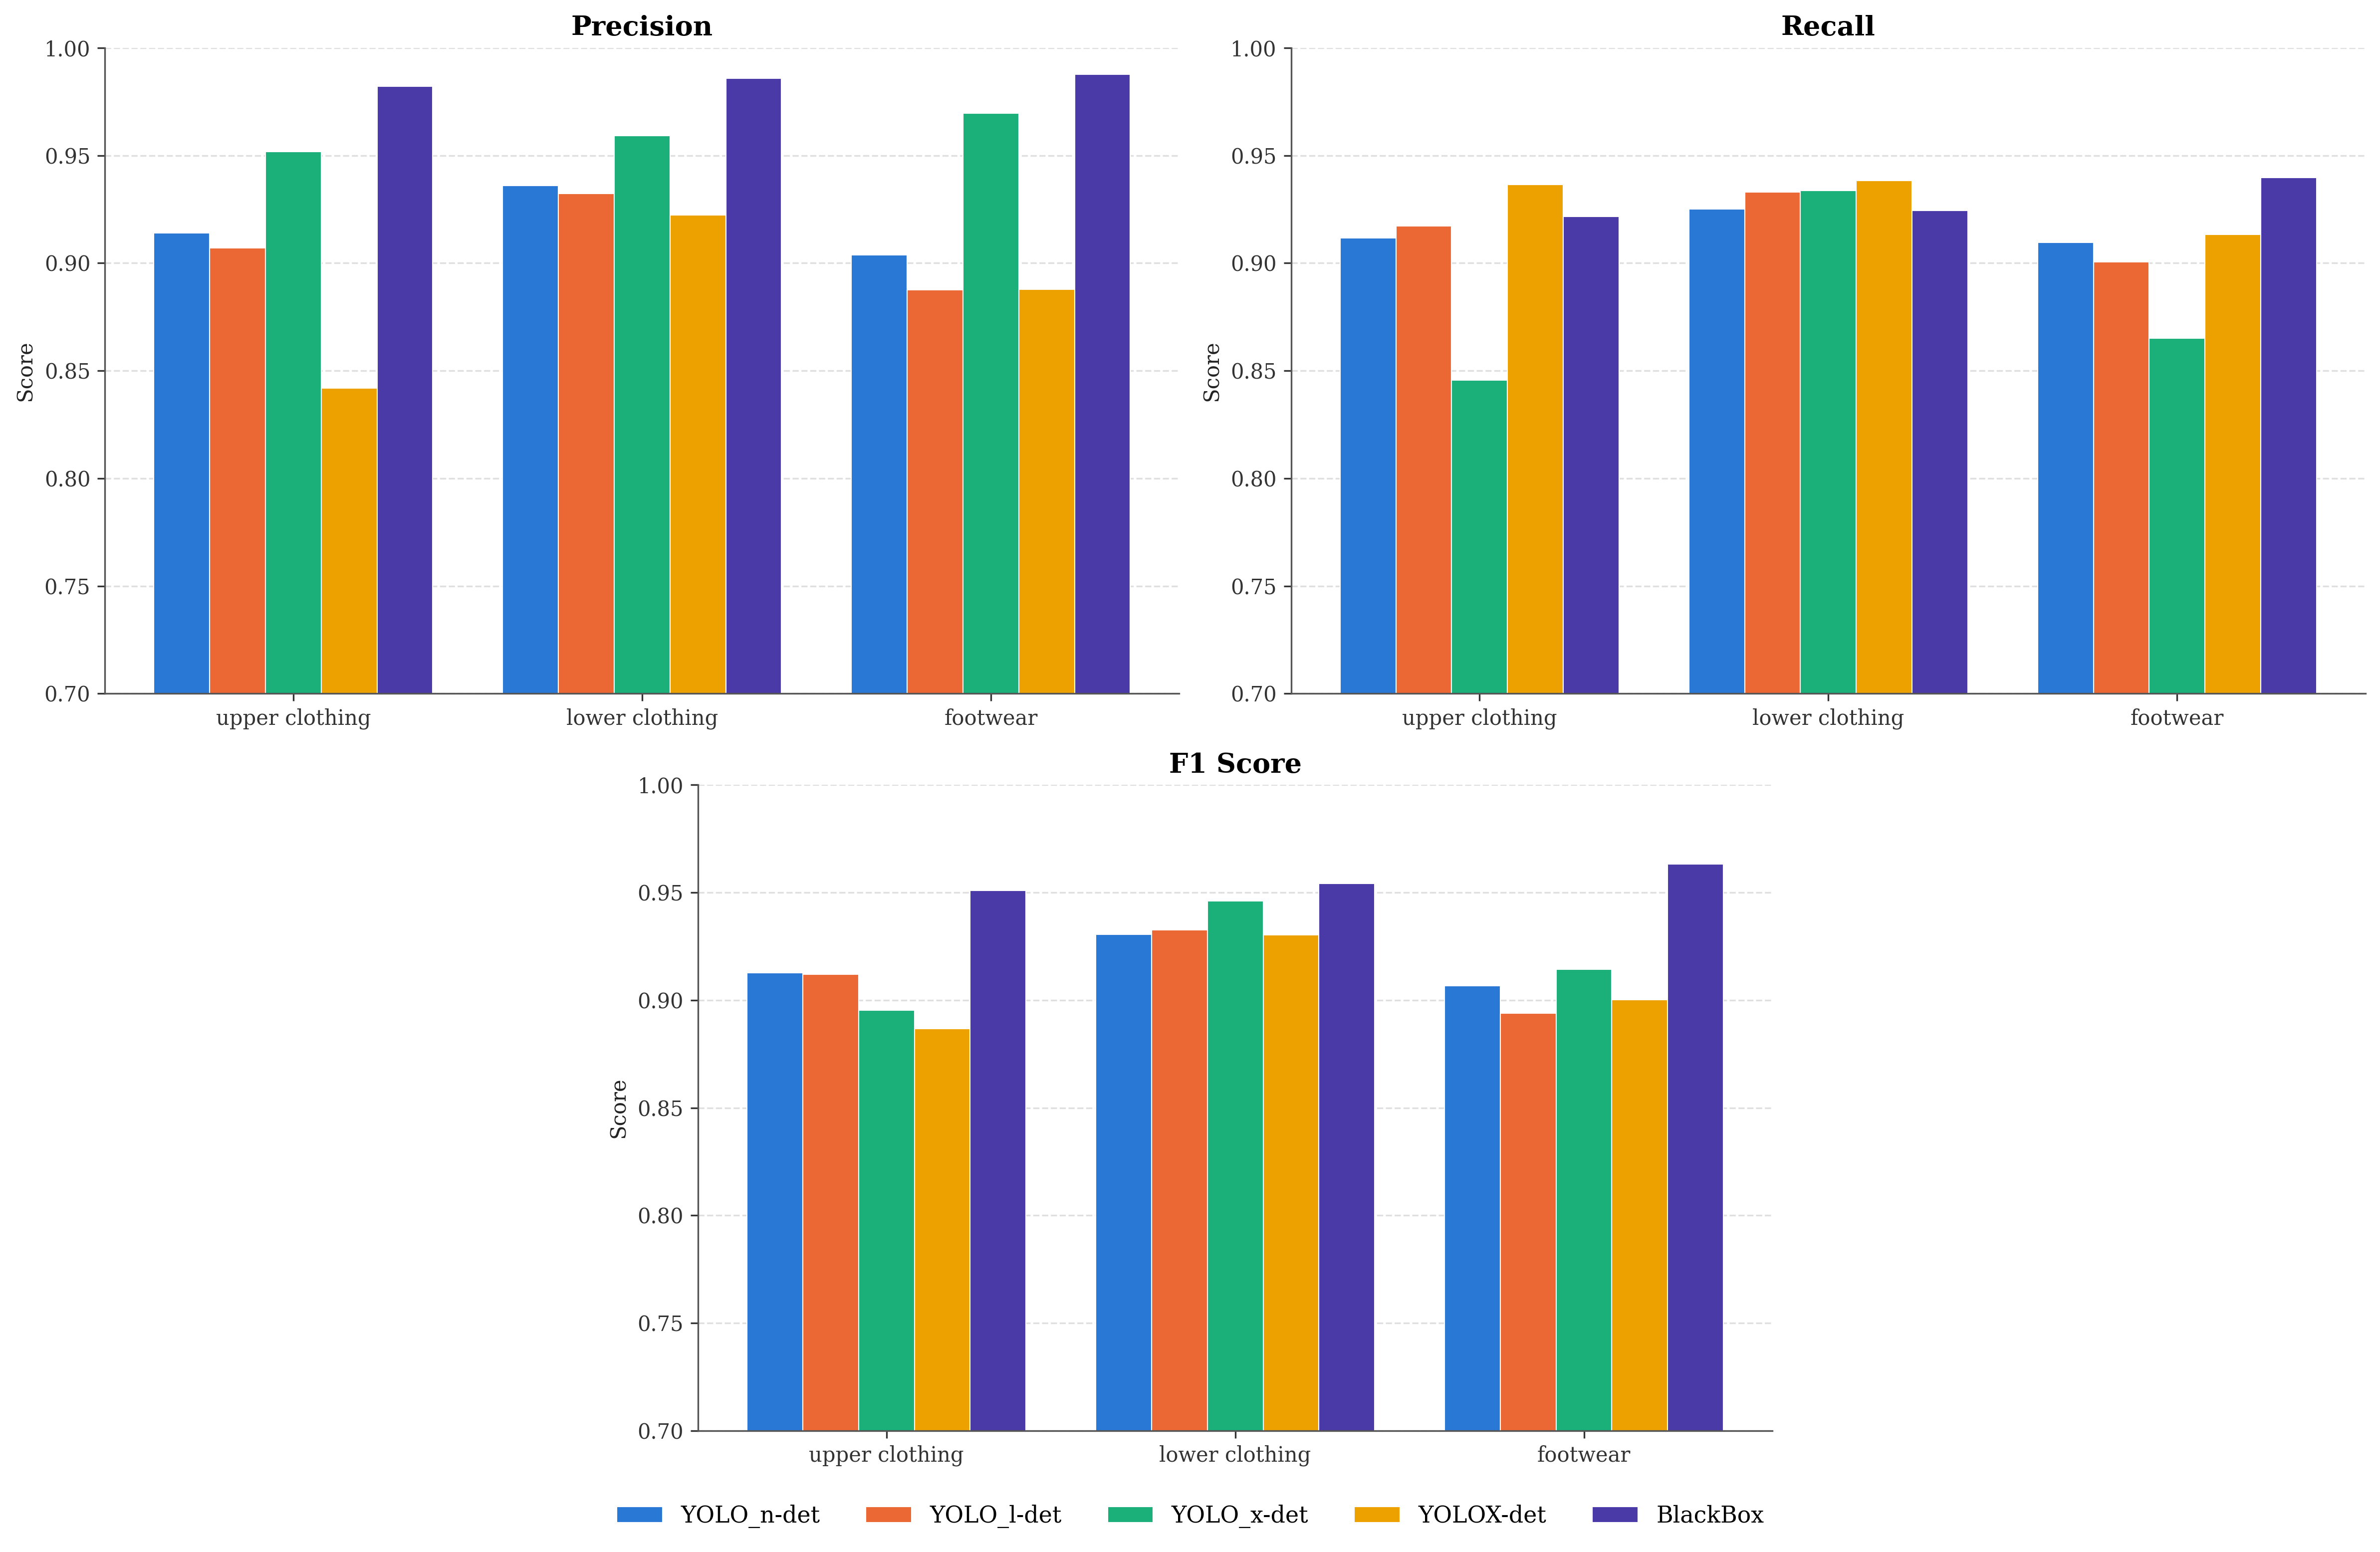
\includegraphics[width=1.2\textwidth]{images/stats/comparison_YOLO_det.png}}
  \label{fig:comparison_YOLO_det}
\end{figure}

\noindent
Come si può osservare, il modello black box mantiene la precision più alta su tutte e tre le classi, con valori vicini a 0.98, e solo YOLO\_x-det riesce ad avvicinarsi a questo risultato, in particolare su \textit{footwear}.
YOLO\_x-det paga però questa precision con una recall sensibilmente più bassa su \textit{upper clothing} e \textit{footwear}, risultando più conservativo: produce poche predizioni errate ma tralascia più oggetti.
YOLOX-det mostra il comportamento opposto, con la recall più alta sulle prime due classi, superiore anche a quella del black box, ma con la precision più bassa, che su \textit{upper clothing} scende a circa 0.84.

\noindent
YOLO\_n-det e YOLO\_l-det si collocano in una posizione intermedia, con precision e recall più bilanciate; da notare che la versione large non supera mai in modo significativo la versione nano.
In termini di F1 score, YOLO\_x-det risulta il più vicino al black box su \textit{lower clothing} e \textit{footwear}, mentre su \textit{upper clothing} viene superato dalle versioni nano e large.

\newpage

\subsection{YOLO segmentation}
Il secondo confronto mette a paragone le varianti di YOLO per la segmentazione, con il miglior modello di detection individuato in precedenza, YOLO\_x-det.

\begin{figure}[htbp]
  \centering
  \makebox[\textwidth][c]{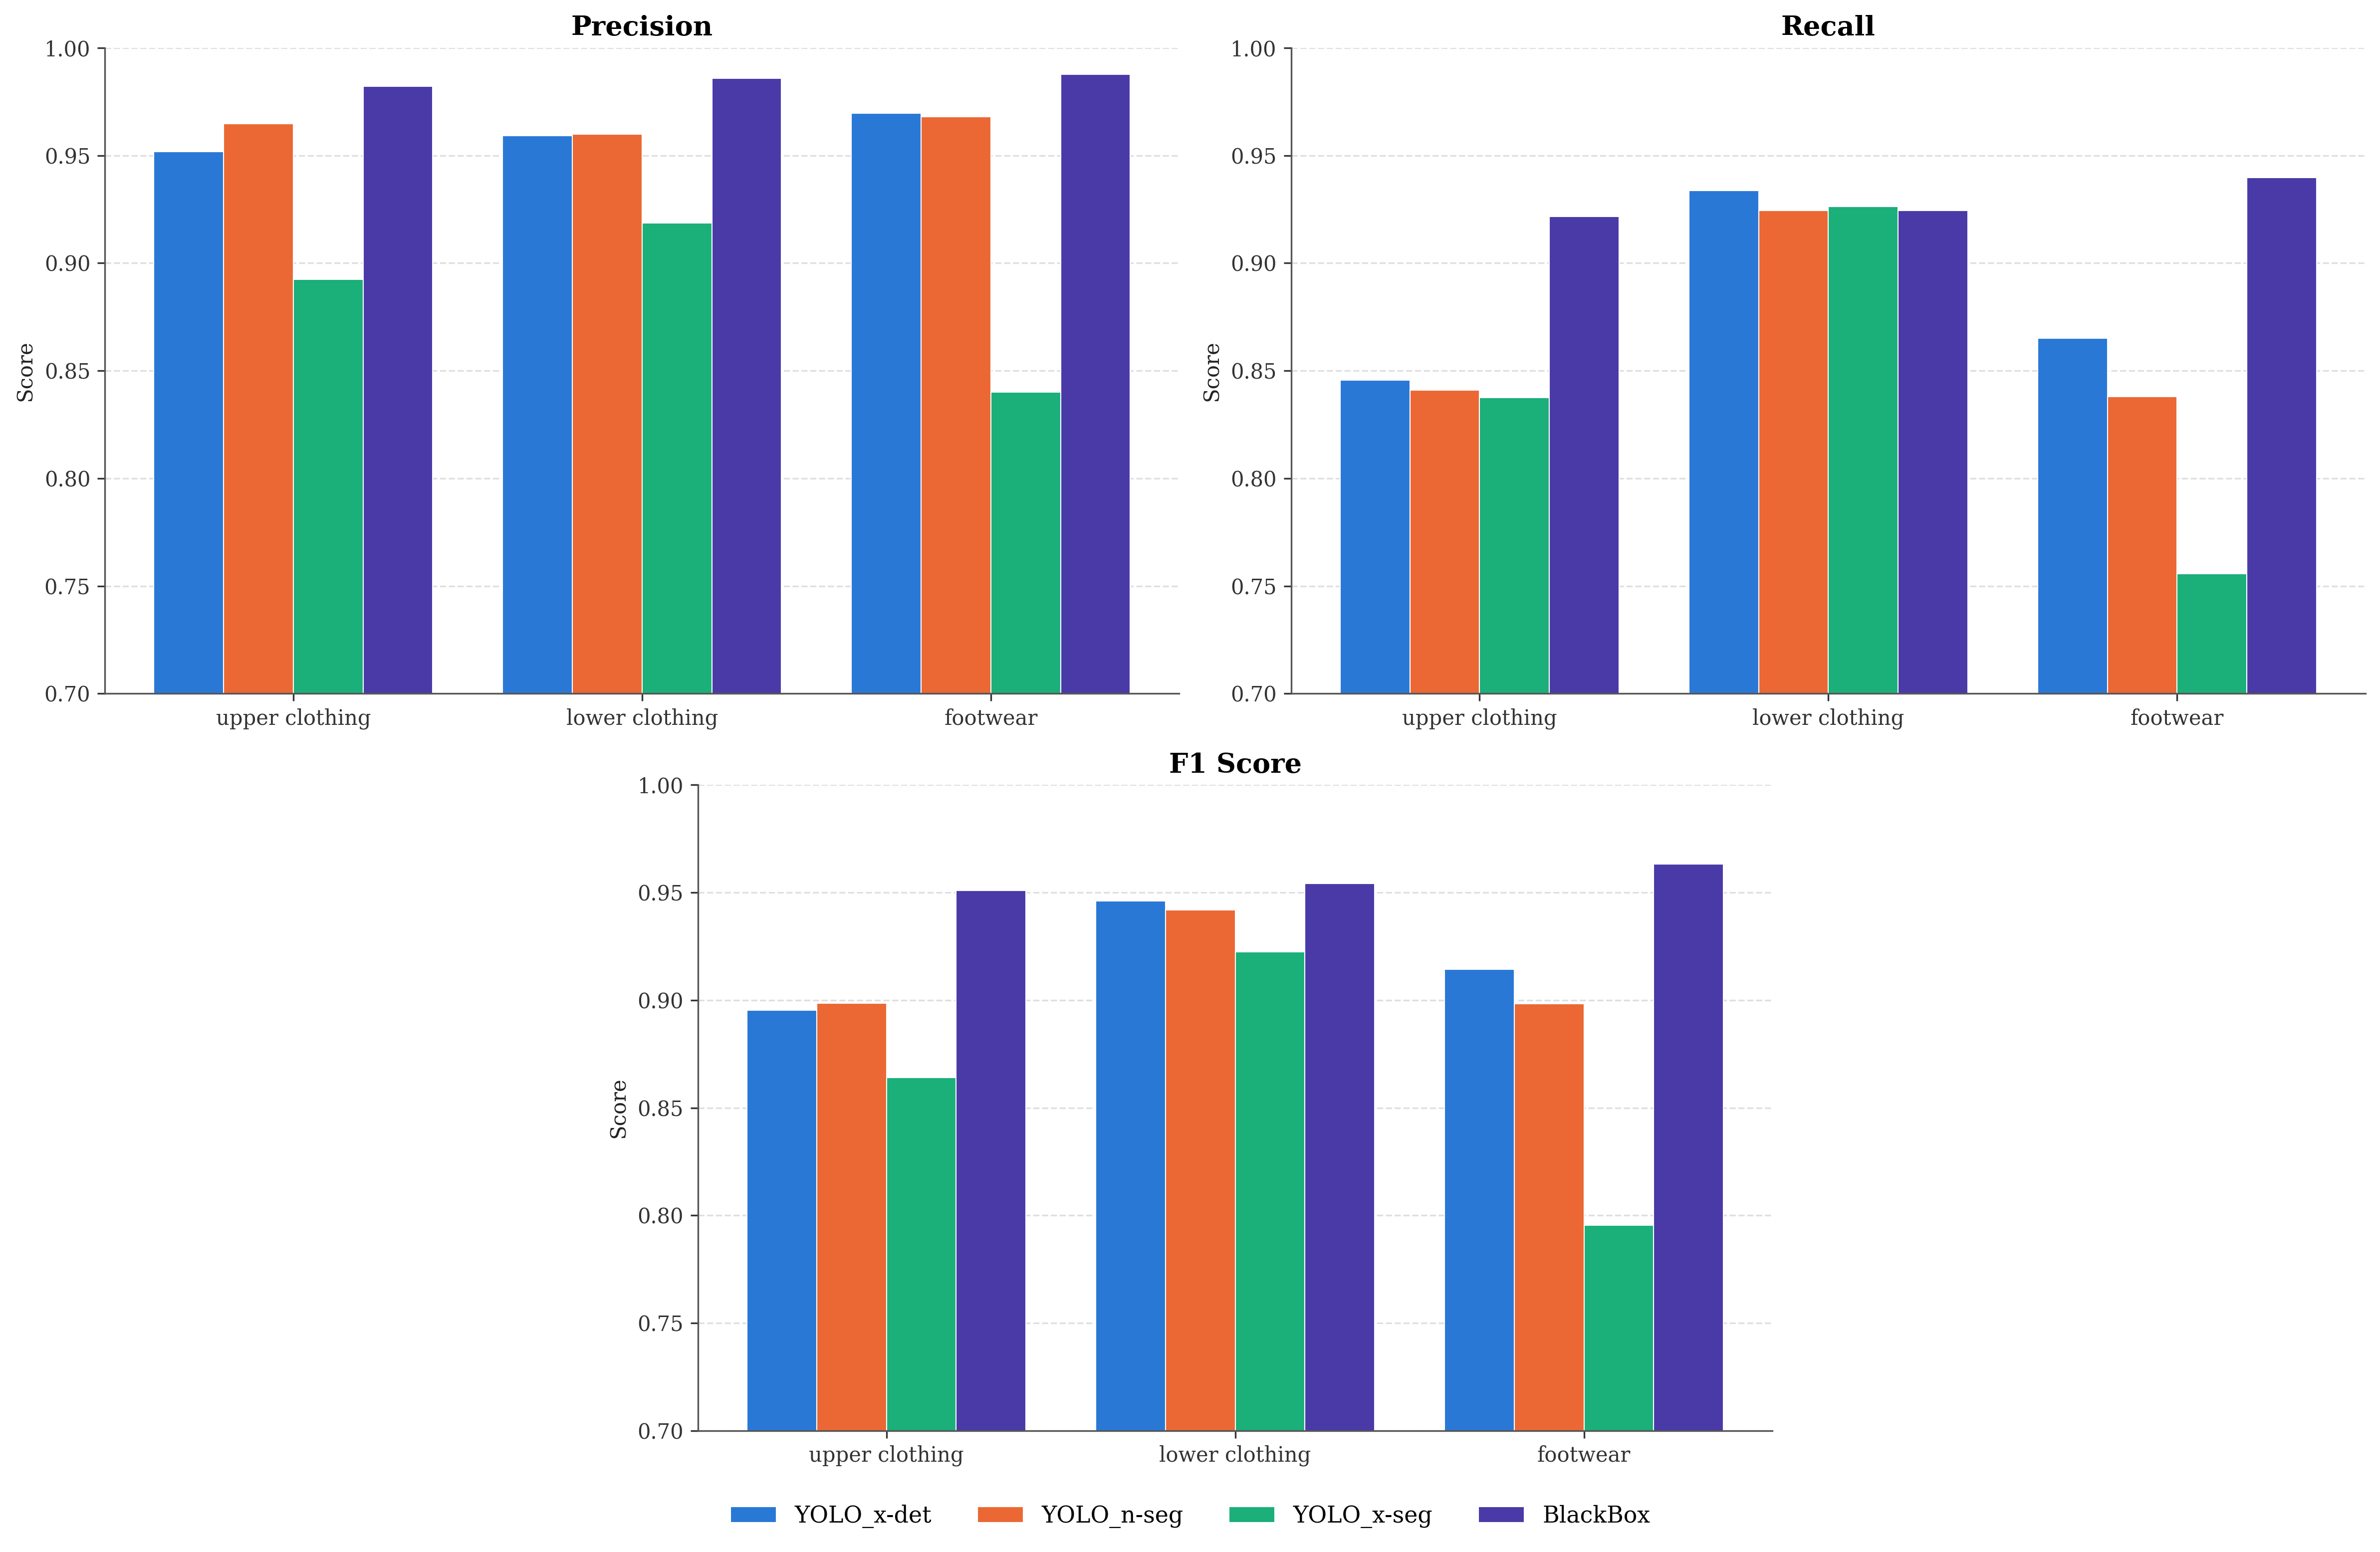
\includegraphics[width=1.2\textwidth]{images/stats/comparison_YOLO_seg.png}}
  \label{fig:comparison_YOLO_seg}
\end{figure}

\noindent
Dal grafico emerge che YOLO\_n-seg ottiene risultati molto simili a YOLO\_x-det: la precision è sostanzialmente la stessa, mentre la recall è di poco inferiore, soprattutto su \textit{footwear}.
Ne deriva un F1 score quasi identico sulle prime due classi e leggermente più basso sulla terza; anche in questo caso, quindi, la versione più piccola del modello si dimostra competitiva.

\noindent
YOLO\_x-seg ha invece prestazioni complessivamente inferiori, in modo evidente su \textit{footwear}, dove la precision si ferma a circa 0.84 e la recall scende intorno a 0.75,
portando l'F1 score sotto 0.80. Le calzature, essendo oggetti piccoli e spesso parzialmente coperti, rappresentano la classe più difficile per questo modello.

\noindent
Tutti e tre i modelli hanno infine una recall su \textit{upper clothing} intorno a 0.84, circa otto punti al di sotto del black box, mentre su \textit{lower clothing} risultano allineati a quest'ultimo.

\newpage

\subsection{SegFormer}
Il terzo confronto riguarda i modelli basati su SegFormer: SegF\_HF e SegF\_StyleMix, confrontati con YOLO\_x-seg.

\begin{figure}[htbp]
  \centering
  \makebox[\textwidth][c]{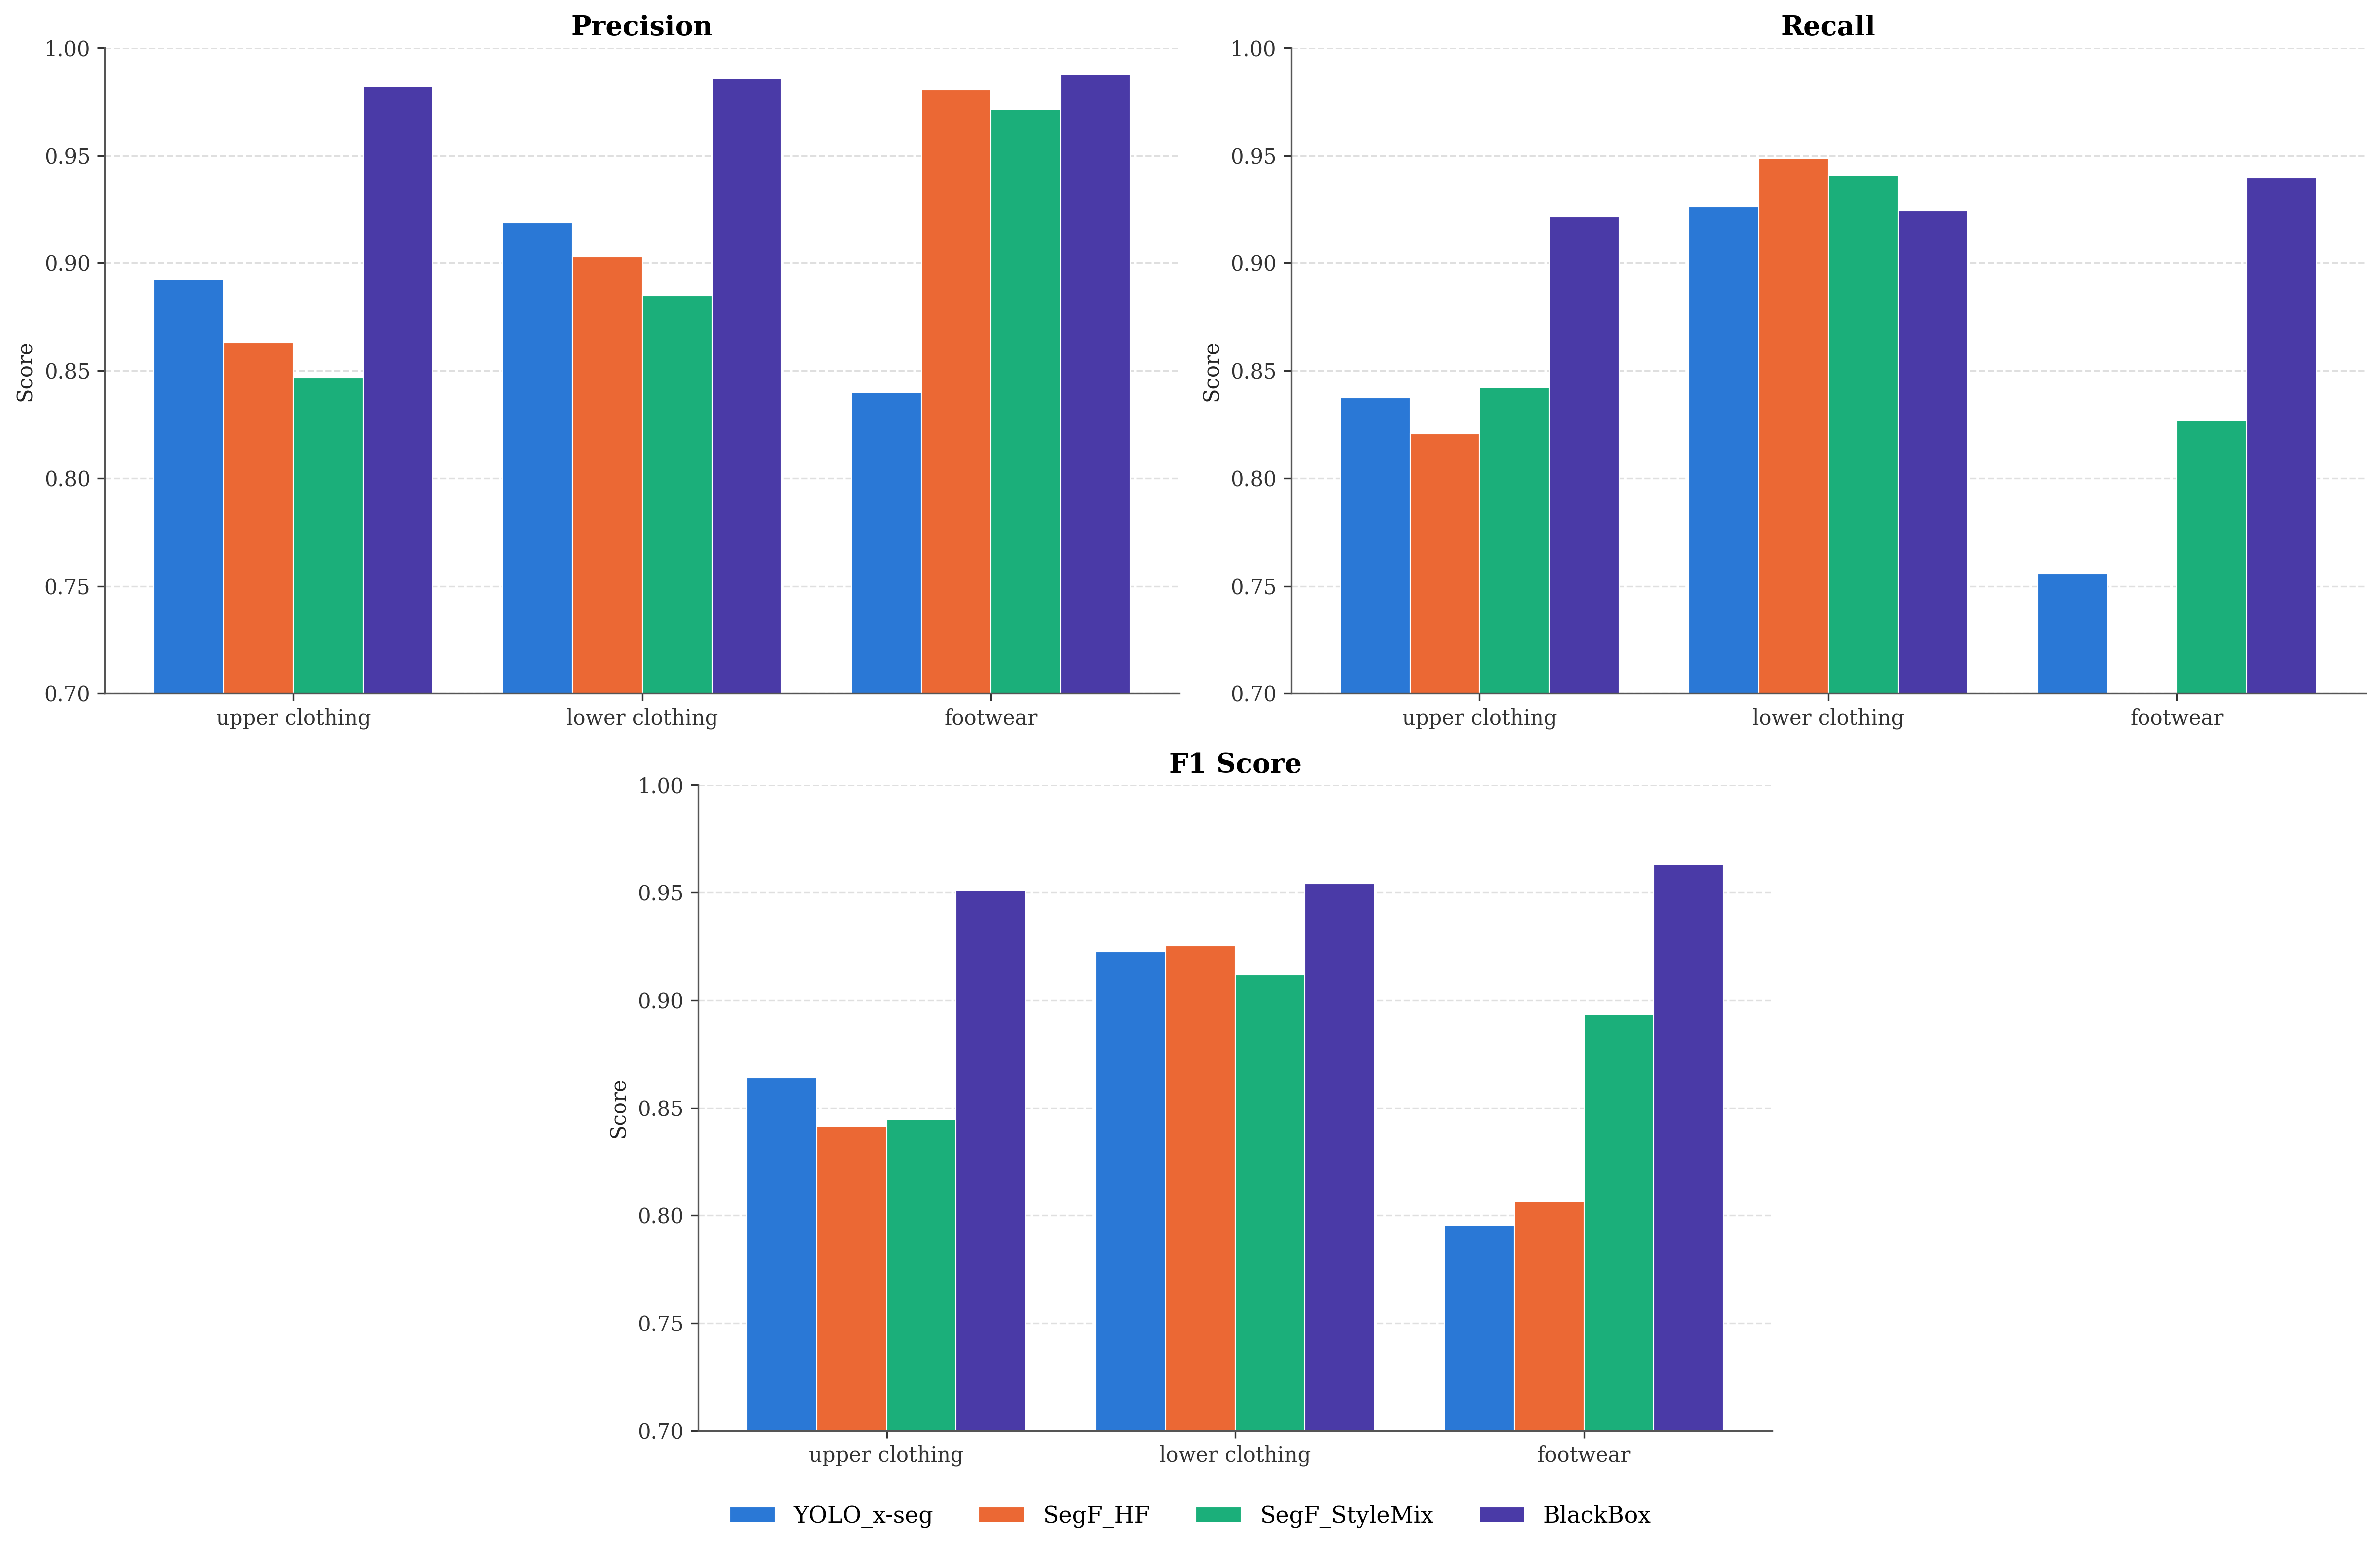
\includegraphics[width=1.2\textwidth]{images/stats/comparison_SegFormer.png}}
  \label{fig:comparison_SegFormer}
\end{figure}

\noindent
In figura si nota come i modelli SegFormer abbiano una precision molto elevata su \textit{footwear}, vicina a quella del black box e nettamente superiore a YOLO\_x-seg.
A questa corrisponde però una recall bassa, che nel caso di SegF\_HF scende al di sotto della scala del grafico: il modello individua con sicurezza le calzature che trova, ma ne tralascia una parte consistente.
SegF\_StyleMix migliora sensibilmente questo aspetto, portando la recall a circa 0.83 e ottenendo su questa classe l'F1 score più alto tra i modelli di segmentazione, pur restando al di sotto del black box.

\noindent
Su \textit{upper clothing} i modelli SegFormer hanno una precision inferiore a YOLO\_x-seg e una recall simile, per cui è quest'ultimo a ottenere l'F1 score migliore.
Su \textit{lower clothing}, invece, raggiungono la recall più alta del grafico, superando anche il black box, ma la precision più bassa mantiene l'F1 score in linea con quello di YOLO\_x-seg.

\newpage

\subsection{GroundingDINO}
Il quarto confronto riguarda i modelli open-vocabulary GroundingDino\_tiny e GroundingDino\_base, confrontati con YOLO\_x-det.

\begin{figure}[htbp]
  \centering
  \makebox[\textwidth][c]{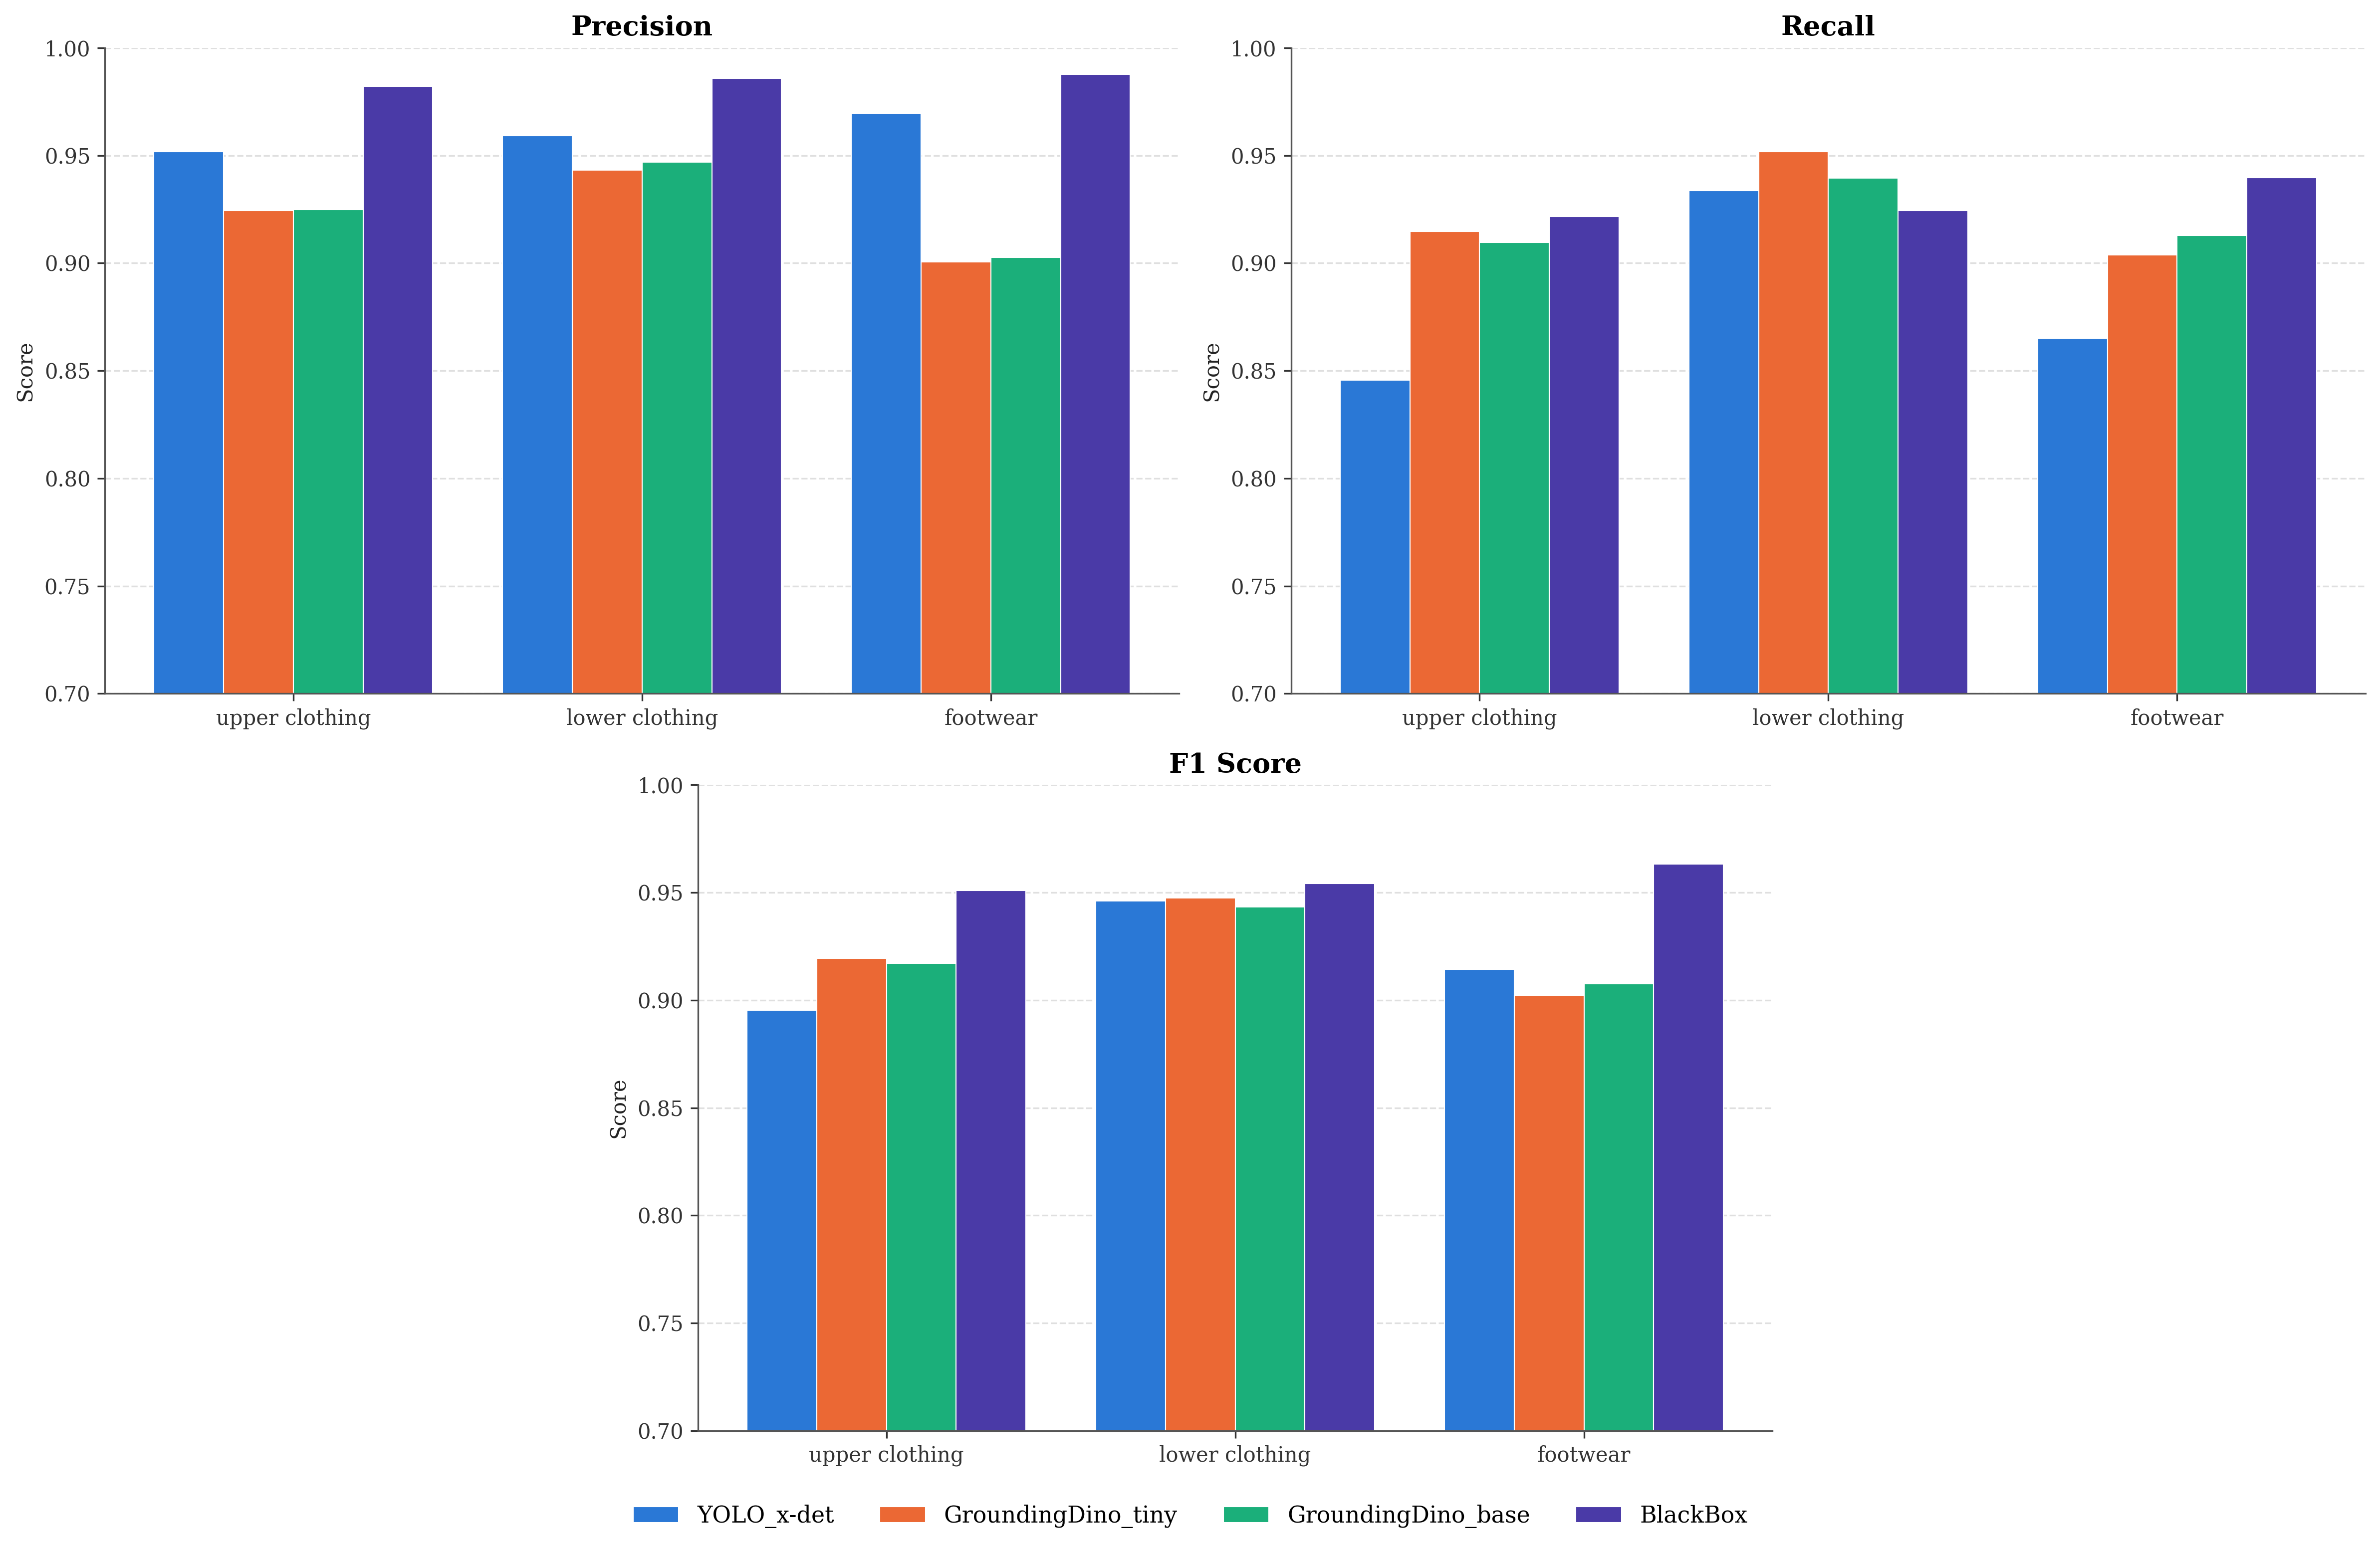
\includegraphics[width=1.2\textwidth]{images/stats/comparison_GroundingDino.png}}
  \label{fig:comparison_GroundingDino}
\end{figure}

\noindent
Come mostrato, entrambe le versioni di GroundingDINO hanno una precision inferiore a YOLO\_x-det su tutte le classi, con un distacco più ampio su \textit{footwear}, dove scendono a circa 0.90 contro 0.97.
In compenso, la recall è più alta su tutte le classi: su \textit{upper clothing} passa da circa 0.85 a 0.91, e su \textit{lower clothing} GroundingDino\_tiny raggiunge circa 0.95, superando anche il black box.

\noindent
Ne risulta un F1 score migliore su \textit{upper clothing}, sostanzialmente equivalente su \textit{lower clothing} e leggermente inferiore su \textit{footwear}, dove il calo di precision non viene compensato del tutto dalla recall.
Le differenze tra la versione tiny e la versione base sono minime, nell'ordine di un punto percentuale o meno: anche in questo caso, un modello più grande non porta vantaggi significativi.

\newpage

\subsection{SAM3}
Infine, abbiamo confrontato SAM3 con i migliori modelli emersi dai confronti precedenti: YOLO\_x-det e SegF\_StyleMix.

\begin{figure}[htbp]
  \centering
  \makebox[\textwidth][c]{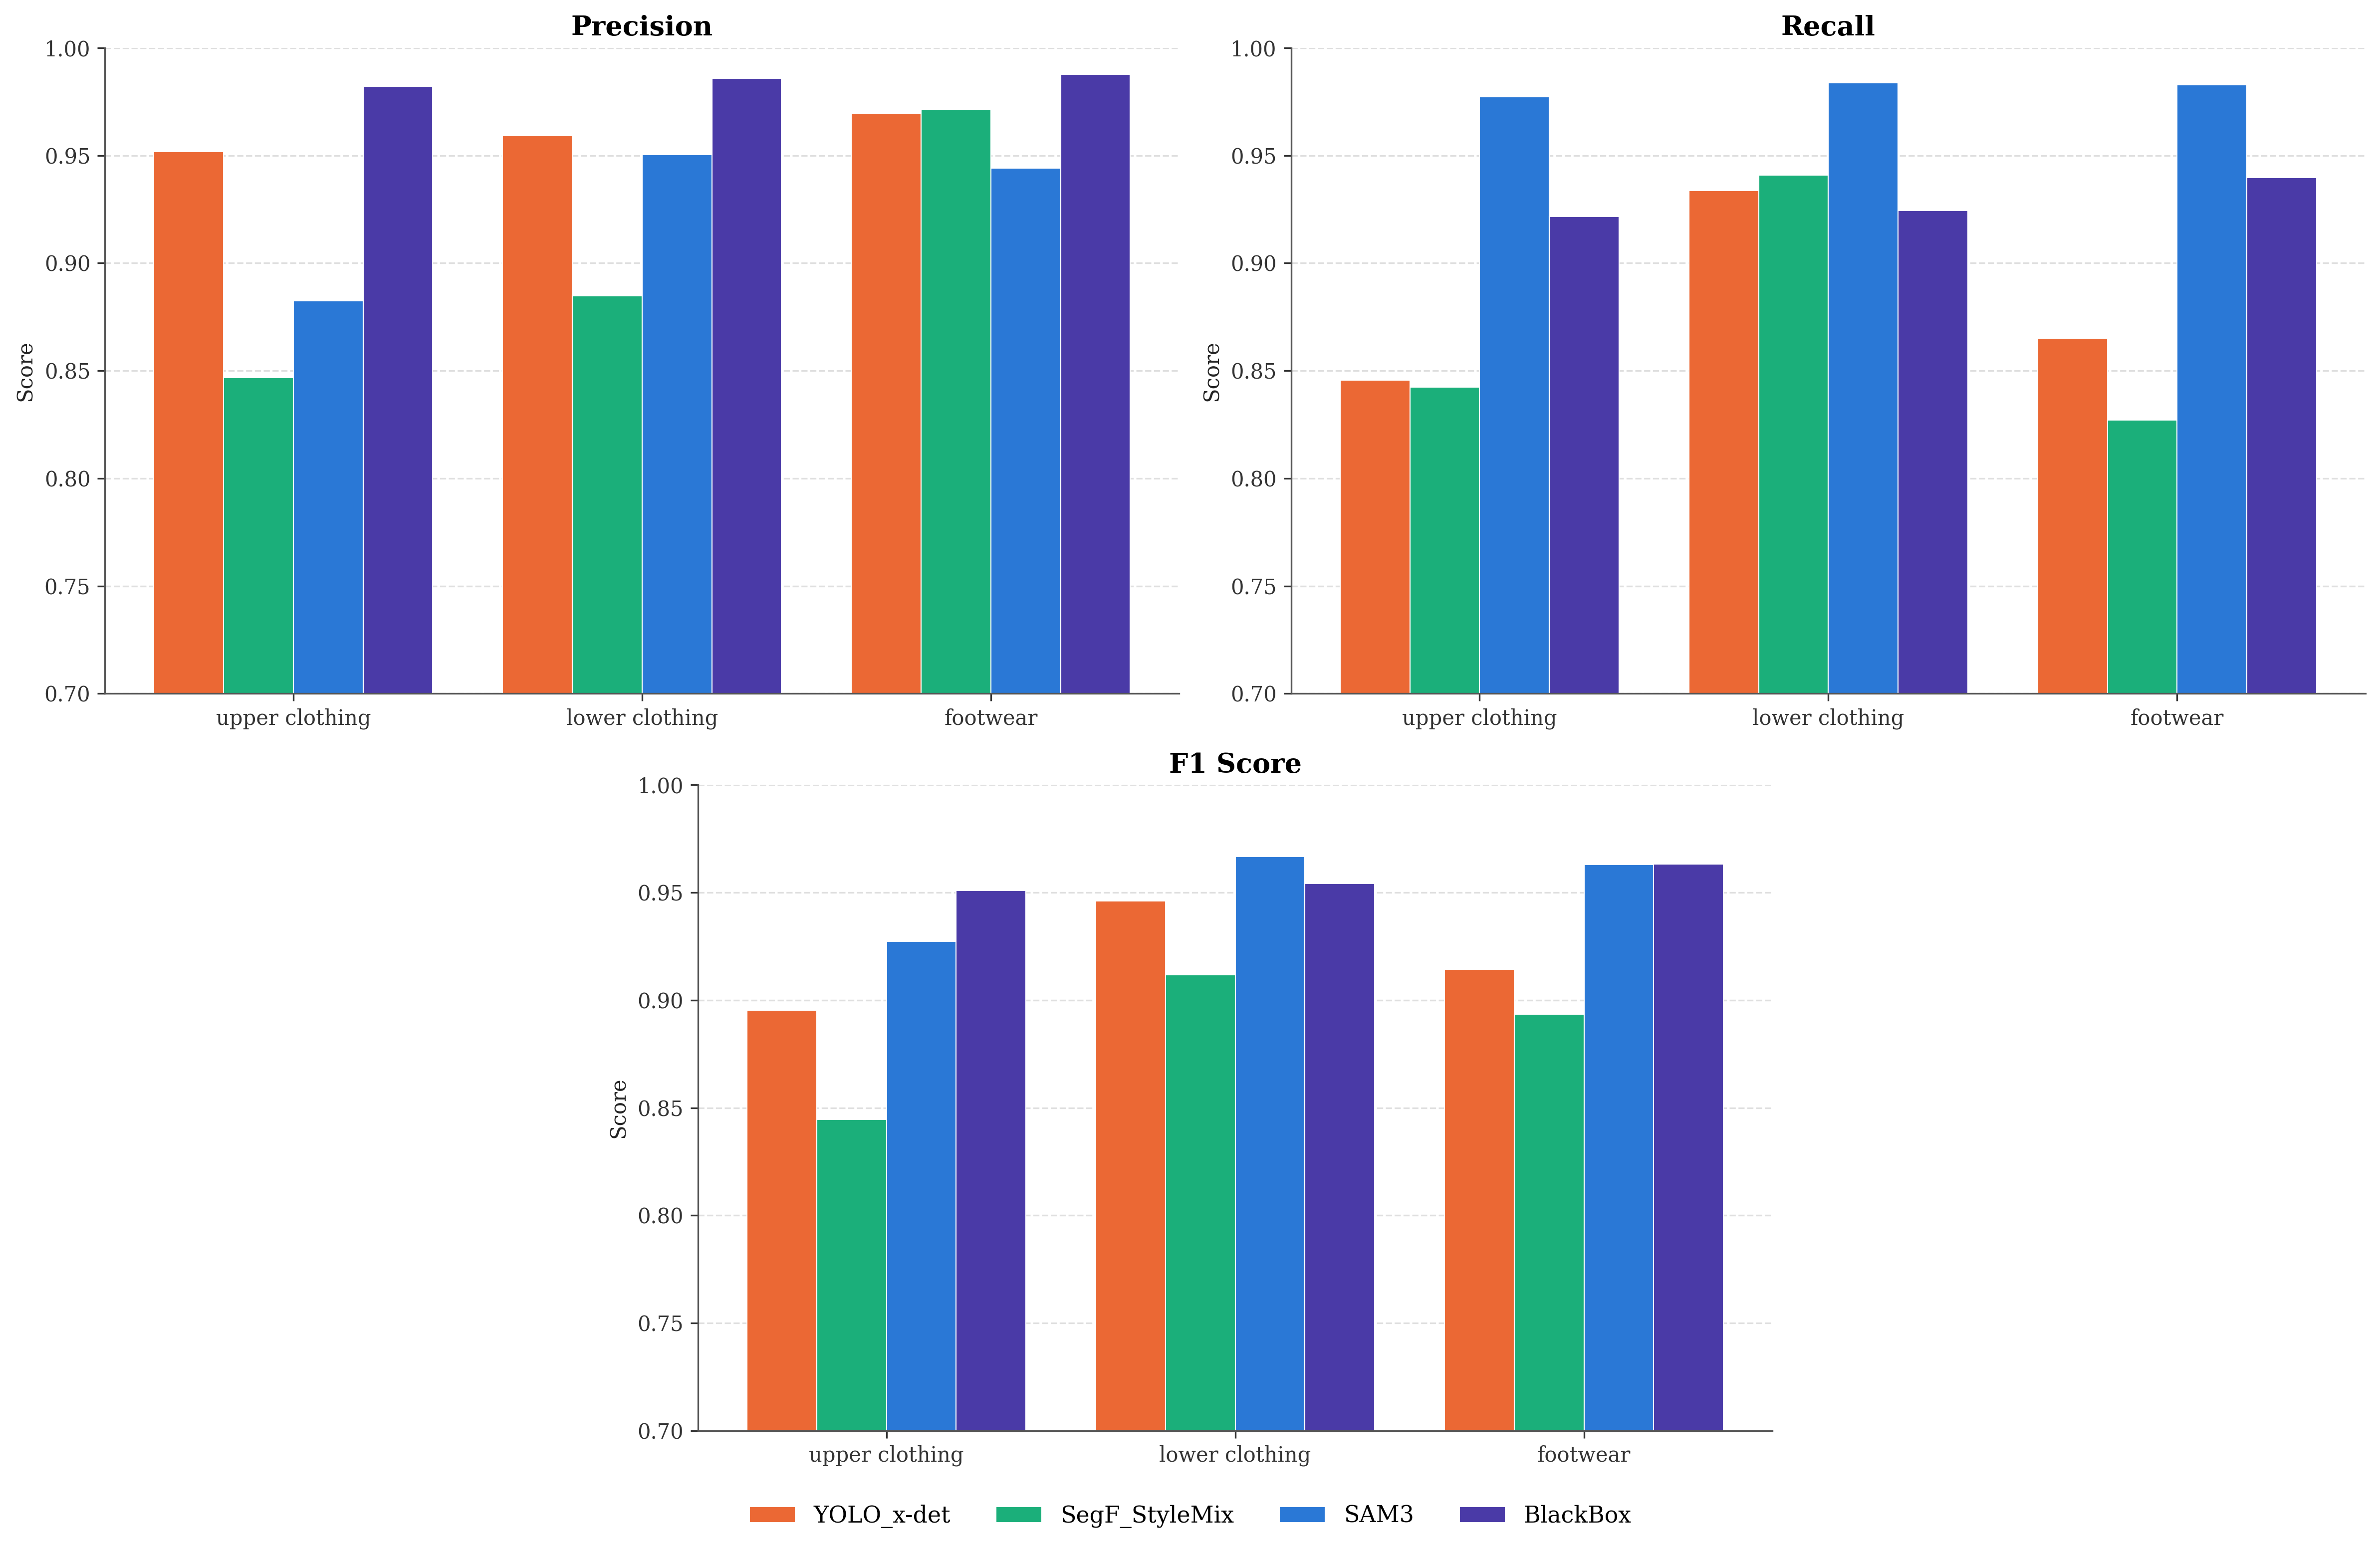
\includegraphics[width=1.2\textwidth]{images/stats/comparison_SAM3_vs_best.png}}
  \label{fig:comparison_SAM3_vs_best}
\end{figure}

\noindent
Qui emerge che SAM3 raggiunge la recall più alta in assoluto, superiore a 0.97 su tutte le classi e quindi anche a quella del black box, che si ferma tra 0.92 e 0.94.
Il vantaggio è particolarmente evidente rispetto a YOLO\_x-det e SegF\_StyleMix su \textit{upper clothing} e \textit{footwear}, dove questi ultimi si fermano intorno a 0.83--0.87.

\noindent
La sua precision resta invece inferiore a quella del black box, con un distacco di circa dieci punti su \textit{upper clothing} e di circa quattro sulle altre due classi.
SAM3 e il black box presentano quindi profili di errore complementari: il primo tende a produrre qualche falso positivo in più, il secondo a tralasciare qualche oggetto.

\noindent
In termini di F1 score, SAM3 supera il black box su \textit{lower clothing}, lo eguaglia su \textit{footwear} e rimane leggermente al di sotto su \textit{upper clothing}.
Ottiene inoltre l'F1 score migliore del confronto su tutte le classi, risultando il modello più vicino al riferimento esterno e l'unico in grado di raggiungerne o superarne le prestazioni su almeno una classe.

\newpage

\section{Dai modelli al sistema}

Il percorso seguito fin qui ha avuto un obiettivo preciso, cioè capire quale fosse lo strumento più adatto a riconoscere i capi d'abbigliamento all'interno di una fotografia.
Dopo aver introdotto i concetti alla base delle reti neurali e del loro addestramento, abbiamo analizzato e addestrato modelli di natura molto diversa, i quali per poterli confrontare in modo equo
abbiamo costruito una ground truth verificata a mano e un protocollo di valutazione comune, che ha permesso di misurarli tutti con lo stesso metro e di metterli a confronto con un modello esterno di riferimento.

Il risultato di questo confronto è stato netto. SAM3 si è rivelato il modello con la recall più alta, in grado di individuare la quasi totalità dei capi presenti nelle immagini,
e l'unico a raggiungere o superare il modello "black box" in termini di F1 score su almeno una classe.
A questo si aggiunge un vantaggio che le metriche non misurano direttamente, SAM3 non richiede alcun addestramento sul nostro dominio, perché viene interrogato in linguaggio naturale,
e può quindi cercare qualunque tipo di capo semplicemente cambiando il prompt testuale.

Riconoscere un capo, però, non è di per sé un risultato utile per l'utente finale. Un modello di segmentazione restituisce maschere e riquadri, cioè informazioni che descrivono una singola immagine,
ma non ci dice nulla sui rapporti tra i prodotti di un catalogo, quali capi vengono indossati insieme, quali stili si abbinano, quale articolo potrebbe completare un outfit.
Per rispondere a domande di questo tipo serve una struttura capace di raccogliere ciò che il modello osserva nelle singole fotografie e di trasformarlo in conoscenza organizzata e interrogabile.

Le fotografie indossate di un catalogo contengono un'informazione implicita molto preziosa: ogni immagine mostra un abbinamento reale, scelto da chi ha curato il catalogo.
Utilizzando SAM3 per isolare i singoli capi presenti in ciascuna fotografia, e riconducendo poi ogni capo all'articolo corrispondente tramite una ricerca per somiglianza visiva, è possibile trasformare queste co-occorrenze in un grafo,
in cui i prodotti sono i nodi e gli abbinamenti osservati sono le relazioni tra di essi.

Il lavoro svolto nei capitoli precedenti non rappresenta quindi un fine a sé stante, ma la base su cui poggia un sistema concreto, cioè l'analisi dei modelli ha permesso di scegliere in modo motivato il componente più affidabile,
e il protocollo di valutazione ha dato una misura oggettiva di quanto ci si possa fidare delle sue predizioni.
Nel prossimo capitolo vedremo come questo componente venga integrato in un'architettura GraphRAG, che affianca un database vettoriale per la ricerca per somiglianza e un database a grafo per la gestione delle relazioni,
dando vita a un sistema in grado di rappresentare e interrogare gli abbinamenti tra i prodotti del catalogo.

\newpage

	\chapter{Graph RAG}

Sebbene la RAG tradizionale sia eccellente nel recuperare documenti basandosi sulla similarità semantica tramite database vettoriali,
si scontra frequentemente con una fisiologica perdita di contesto. I modelli vettoriali, infatti, faticano nel multi-hop reasoning,
ovvero nella capacità di estrarre e dedurre relazioni tra concetti distanti all'interno di un vasto corpus documentale.
Questo porta spesso a risposte incomplete o fuorvianti, specialmente quando le connessioni tra le informazioni non sono esplicitate nel testo.

Per arginare questo problema, è stato formalizzato il concetto di GraphRAG, un paradigma che sostituisce o affianca i vettori ai Knowledge Graph (KGs),
permettendo così di mappare in modo esplicito le entità e le loro interrelazioni. Tuttavia, l'implementazione originale di GraphRAG si rivela fortemente
"LLM-centrica", introducendo nuove criticità architetturali. Demandare a un Large Language Model l'intera costruzione del grafo e la sua successiva interrogazione —
ad esempio costringendolo a tradurre a runtime il linguaggio naturale in query Cypher — espone il sistema al rischio di allucinazioni sintattiche,
inconsistenze ontologiche e a un'impennata insostenibile dei costi di inferenza su larga scala.

La soluzione ingegneristica proposta supera questi colli di bottiglia integrando un database vettoriale (Qdrant) con un database a grafo (Neo4j),
facendoli comunicare attraverso la condivisione di identificatori univoci.

\newpage

\noindent
Il ciclo di vita del dato all'interno di questo sistema si divide in due macro-fasi. Durante l'inserimento dei dati (Ingestion),
i testi grezzi vengono elaborati — tramite LLM o tecniche di Named Entity Recognition — per estrarne un'ontologia strutturata di entità e relazioni,
che viene archiviata nel database a grafo Neo4j. Parallelamente, gli stessi documenti vengono convertiti in embedding vettoriali e memorizzati in Qdrant.
In questo modo, il sistema si assicura che la medesima informazione sia esplorabile sia da un punto di vista puramente semantico sia strutturale.

La vera sinergia tra le due tecnologie si esprime nella fase di recupero e generazione (Retrieval \& Generation). Quando l'utente pone una domanda,
il sistema non cerca di tradurla direttamente in linguaggio per i grafi, ma esegue prima una veloce ricerca vettoriale su Qdrant.
Questo passaggio permette di isolare in modo efficiente i frammenti di testo semanticamente più pertinenti. Una volta ottenuti gli ID di questi documenti,
il sistema li utilizza come punto di ingresso per interrogare Neo4j: il database a grafo recupera le reti relazionali associate a quegli ID,
espandendo il contesto con i nodi adiacenti e le loro connessioni esplicite.

\begin{figure}[htbp]
  \centering
  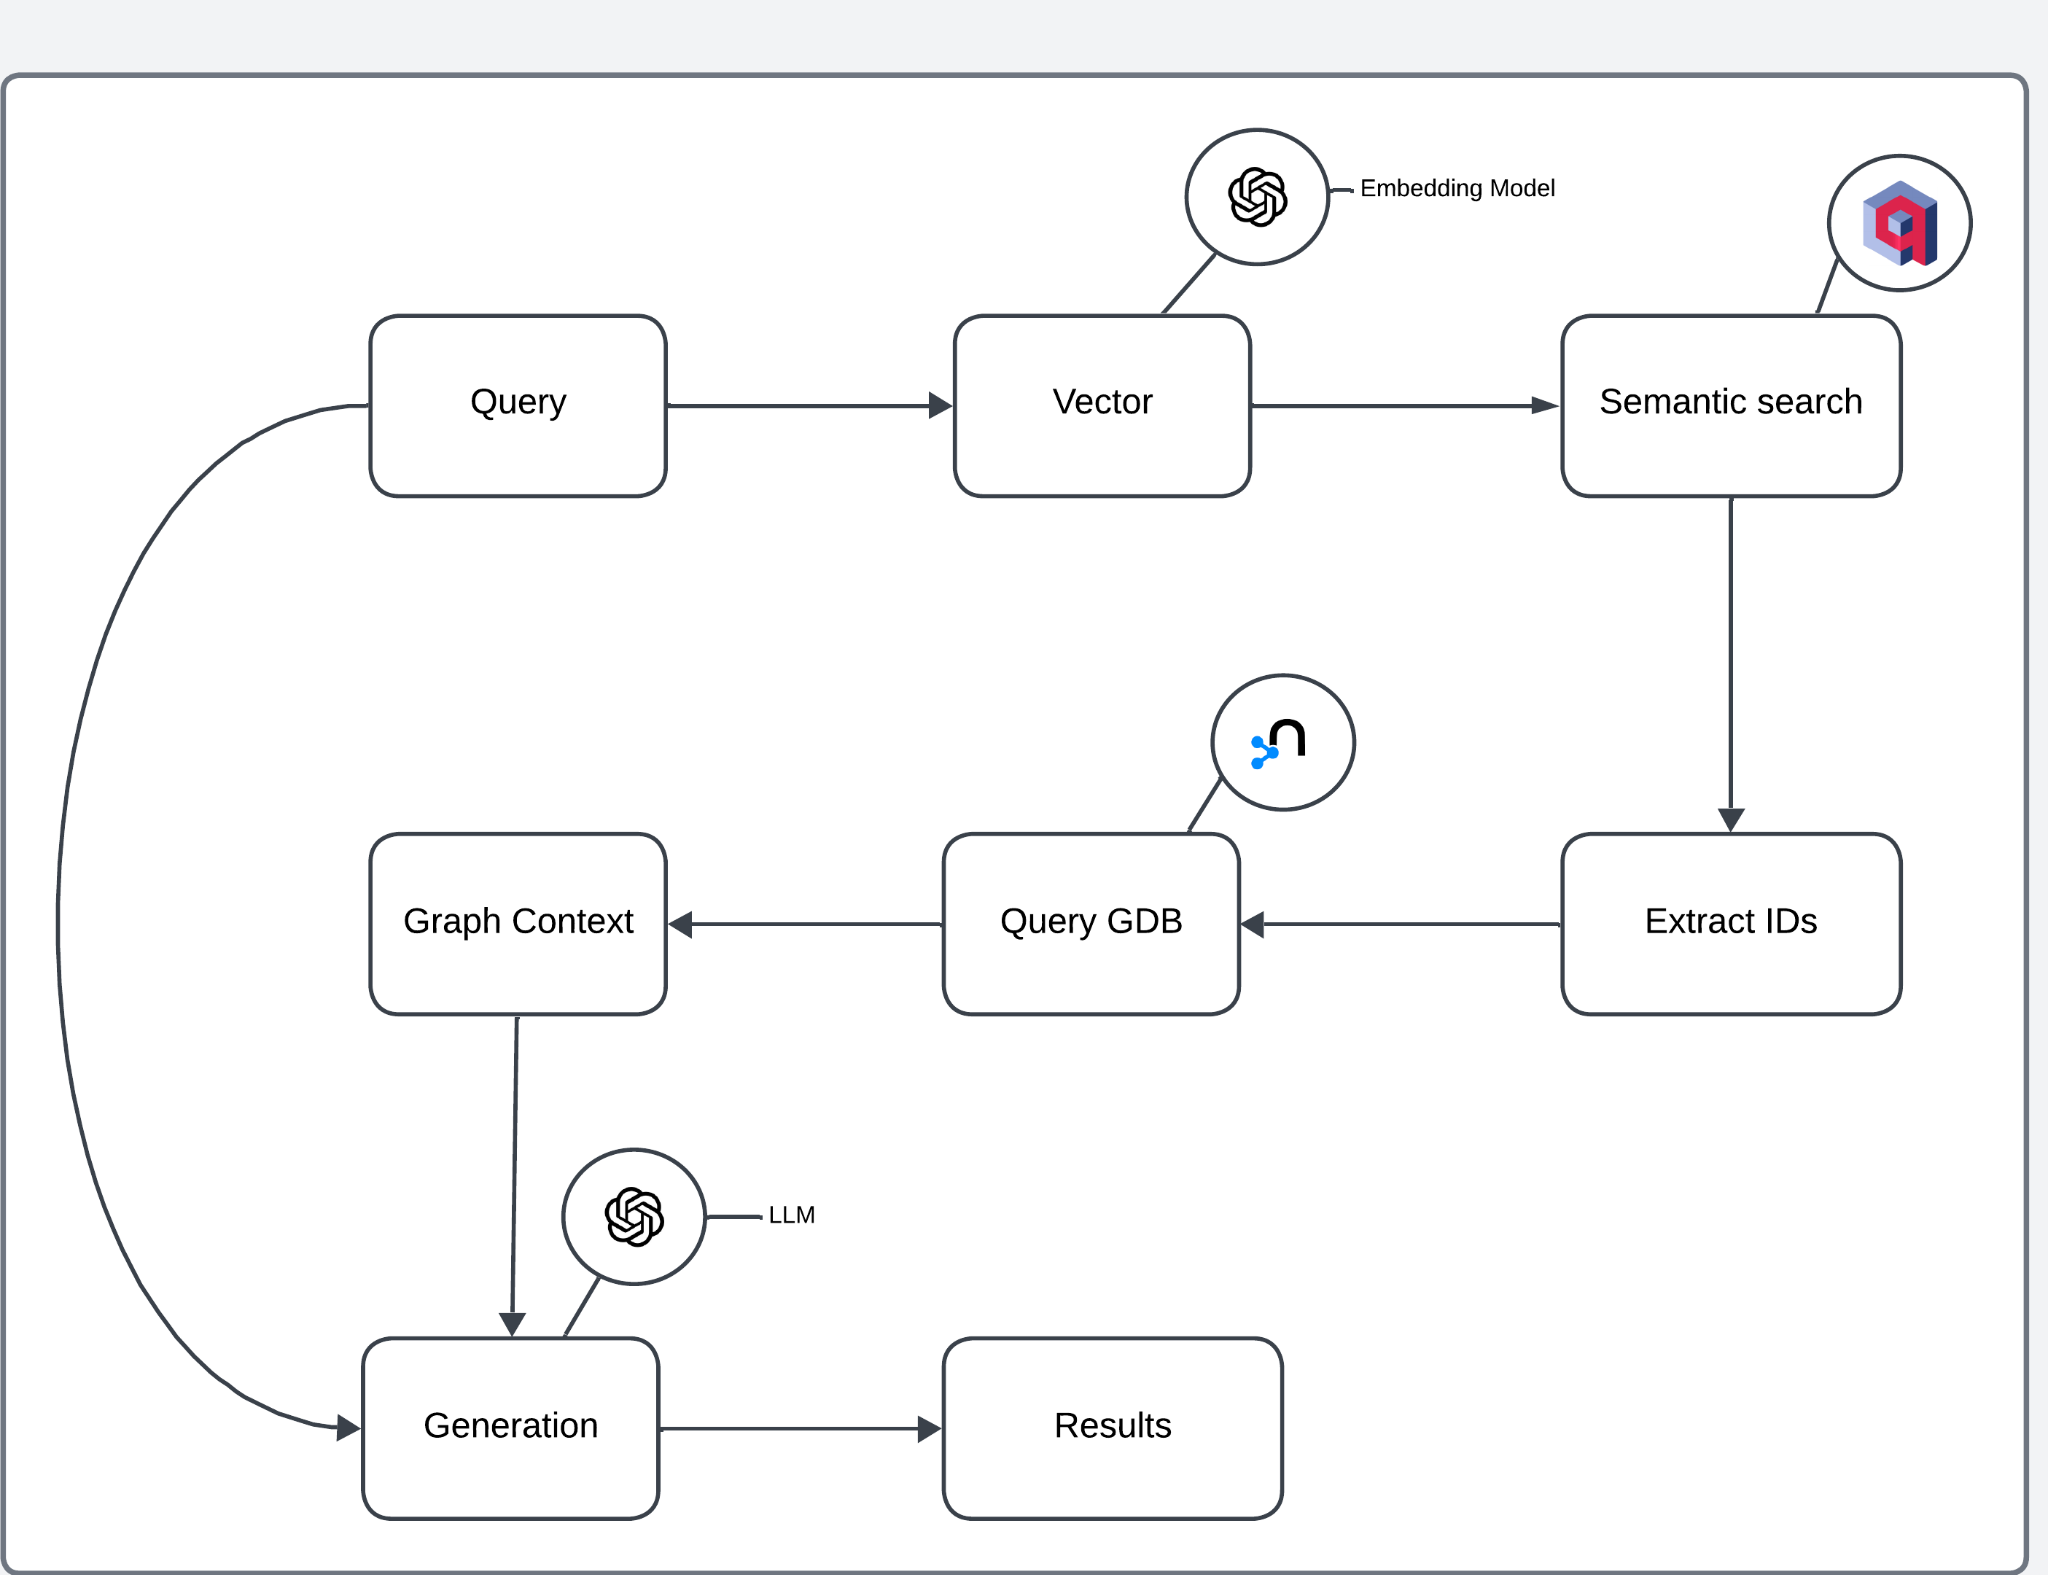
\includegraphics[width=0.7\textwidth]{images/graph_rag.png}
  \caption{grafo RAG}
  \label{fig:graph RAG}
\end{figure}

\noindent
Il risultato finale è un contesto ibrido, denso e deterministico, che viene fornito all'LLM per la generazione della risposta.
In un'ottica di architettura del software, il valore centrale di questo approccio per una tesi di informatica risiede nel principio di disaccoppiamento
delle responsabilità. Qdrant gestisce agilmente il matching semantico, Neo4j garantisce il rigore del contesto relazionale e l'LLM viene sollevato dal ruolo
inappropriato di "motore di interrogazione", tornando a fungere esclusivamente da generatore linguistico. Questo paradigma ibrido abbatte i costi computazionali,
azzera gli errori di querying dinamico e garantisce un'affidabilità delle risposte notevolmente superiore rispetto agli approcci monolitici. \cite{graph_rag}

\newpage

\section{Database vettoriali}
I database vettoriali rappresentano un'evoluzione fondamentale per l'Intelligenza Artificiale moderna. Essi sono progettati per memorizzare,
indicizzare e interrogare dati rappresentati sotto forma di embedding, ovvero vettori numerici ad alta dimensionalità generati da modelli di machine learning.
A differenza dei tradizionali motori di ricerca basati su keyword matching, i vector database operano attraverso la ricerca per similarità spaziale
(es. similarità del coseno, distanza euclidea o prodotto interno). Due concetti semanticamente affini si troveranno vicini all'interno dello spazio vettoriale,
indipendentemente dai termini specifici utilizzati per descriverli.

Nel contesto della nostra architettura, Qdrant ricopre l'incarico cruciale di motore di Semantic Search. Il suo compito è elaborare dati originariamente
non strutturati (es. le descrizioni in linguaggio naturale dei prodotti) e mapparli vettorialmente. Quando il sistema riceve una query,
Qdrant agisce come primo livello di filtraggio: isola in tempi dell'ordine dei millisecondi i frammenti informativi o i prodotti che presentano
la maggiore vicinanza semantica alla richiesta dell'utente. Qdrant eccelle nel gestire l'ambiguità del linguaggio naturale, individuando il "punto di ingresso"
ideale per la ricerca, ma, per sua natura, non possiede la consapevolezza strutturale di come tali informazioni siano collegate tra loro in un dominio complesso.

\section{Database a Grafo}
Per sopperire alla mancanza di contesto relazionale dei vettori, entrano in gioco i database a grafo. Questa tecnologia basa la propria architettura
sulla teoria dei grafi, abbandonando il rigido schema a tabelle dei database relazionali per modellare l'informazione attraverso nodi (le entità fisiche o logiche),
archi (le relazioni esplicite che collegano le entità) e proprietà. Il paradigma a grafo eccelle laddovebil valore dell'informazione risiede primariamente
nelle interconnessioni tra i dati.

Nel nostro sistema, Neo4j costituisce l'ossatura logica e relazionale dell'applicazione. A valle del processo di estrazione (operato da modelli come SAM3),
Neo4j immagazzina l'ontologia del dominio: istanzia i prodotti come nodi e crea un reticolo denso di archi che ne definiscono categorie, compatibilità,
specifiche tecniche e logiche di accoppiamento. Il principale vantaggio prestazionale di Neo4j è l'elaborazione Index-Free Adjacency:
le operazioni di attraversamento del grafo avvengono in tempo reale, poiché ogni nodo mantiene puntatori fisici diretti ai nodi adiacenti.
Ciò rende Neo4j lo strumento perfetto per il multi-hop reasoning, ovvero la capacità di estrarre percorsi logici complessi con una latenza minima,
indipendente dalle dimensioni totali del database.

\section{Integrazione di SAM3}

Come discusso in precedenza in merito all'architettura ibrida, il modello SAM3 svolge un ruolo cruciale all'interno del sistema,
fungendo da motore d'inferenza principale per la fase di popolamento (o ingestion) del database a grafo, che in questa implementazione è Neo4j.
Nello specifico, le avanzate capacità di analisi di SAM3 vengono impiegate per processare i dati in ingresso ed estrarre, con un elevato grado di precisione,
tutte le entità e le caratteristiche salienti pertinenti al dominio applicativo in esame.

Questo processo di estrazione mirata permette di tradurre informazioni eterogenee in un'ontologia ben definita e pronta per l'archiviazione strutturata.
Una volta isolati, gli elementi estratti vengono mappati e memorizzati all'interno dell'istanza di Neo4j: i prodotti di interesse vengono istanziati sotto forma
di nodi, mentre le loro peculiarità, i metadati e le reciproche interdipendenze vanno a costituire gli archi (relazioni).
Questa mappatura sistematica e deterministica porta alla generazione di un catalogo prodotti completo e semanticamente interconnesso,
sfruttando a pieno i vantaggi di flessibilità e modellazione offerti da Neo4j rispetto ai tradizionali database relazionali.

La strutturazione dell'informazione all'interno di un property graph come Neo4j apre a scenari di elaborazione e interrogazione particolarmente avanzati.
In fase di ricerca (retrieval), il sistema è in grado di avvalersi della topologia della rete, permettendo di navigare le relazioni esplicite
— anche attraversando nodi multipli — per rispondere a query complesse con latenze estremamente ridotte.
Inoltre, l'adozione di Neo4j si rivela fondamentale per l'implementazione di logiche di "accoppiamento significativo". Analizzando i percorsi, le adiacenze
e i gradi di separazione tra i vari nodi, il sistema può dedurre connessioni semantiche non banali tra molteplici prodotti. Ciò abilita lo sviluppo di funzionalità
di alto livello, come i sistemi di raccomandazione context-aware, capaci di suggerire combinazioni di articoli basate su affinità strutturali e logiche di business
codificate direttamente all'interno della rete relazionale del grafo.
	
	\printbibliography[heading=bibintoc, title={Bibliografia}]
	
\end{document}